\documentclass{article}
\usepackage[utf8]{inputenc}
\usepackage{geometry} % Add geometry package here
\geometry{margin=1.2in} % Set the margin size here
\usepackage{listings}
\usepackage{fancyhdr}
\usepackage{amssymb}
\usepackage{amsmath}
\usepackage{graphicx}
\usepackage{xcolor}
\usepackage{pgfplots}
\usepackage{float}
\usepackage{algorithm}
\usepackage{algpseudocode}
\usepackage[backend=biber]{biblatex}
\usepackage{hyperref}

\hypersetup{citecolor=blue}

\addbibresource{sources.bib}

\pgfplotsset{compat=1.16}

\graphicspath{ {./images/} }

\hypersetup{
    colorlinks=true,
    linkcolor=blue,
    pdfpagemode=FullScreen,
}

\definecolor{code-gray}{RGB}{220, 220, 220}

\pagestyle{fancy}
\fancyhf{}
\fancyfoot[LE,RO]{\thepage}

\lstset{
  basicstyle=\ttfamily,
  columns=fullflexible,
  frame=single,
  breaklines=true,
  showstringspaces=false,
  backgroundcolor=\color{code-gray}
}

\renewcommand{\headrulewidth}{1pt}
\renewcommand{\footrulewidth}{1pt}


\begin{document}

\begin{titlepage}
  \begin{center}
      \vspace*{1cm}

      \LARGE
      \textbf{Diffusion Models in Depth: From a Theoretical and a Practical Perspective}

      \vspace{1.5cm}

      \Large
      \textbf{Gregory Igor Sedykh}
      \vspace{0.8cm}

      \normalsize
      June 28th 2024

      \vfill

      
\includegraphics[width=0.4\textwidth]{images/informatics_en.png} \\

      Bachelor thesis for the degree of Bachelor of Science in Computer Science \\
      Supervised by Prof. Stéphane Marchand-Maillet     

      \vspace{0.8cm}
    
           
           
  \end{center}
\end{titlepage}

\pagenumbering{roman}
\newpage
\section*{Abstract}

\newpage
\tableofcontents

\pagenumbering{arabic}

%% ----------------------- Content goes here ----------------------- %%

\newpage
\section{Introduction}

Diffusion models have gained widespread popularity since 2020, as models such as DALL-E, Stable Diffusion and Midjourney have proven to be capable of generating high-quality images given a text prompt. Furthermore, OpenAI's recent announcement of Sora has shown that diffusion models have now also become highly capable of generating minute long high-definition videos from a text prompt. \cite{videoworldsimulators2024}
\\\\
These models date back to 2015, where the idea of a diffusion model appeared, based on diffusion processes used in thermodynamics. \cite{sohldickstein2015deep} \\
Denoising Diffusion Probabilistic Models (DDPMs) were a development of the original diffusion probabilistic model introduced in 2015. \cite{ho2020denoising} \\
Subsequently, OpenAI improved upon the original DDPMs which did not have ideal log likelihoods \cite{ho2020denoising} while also using less forward passes and therefore speeding up the sampling process. \cite{nichol2021improved} \\
The most recent progress done by OpenAI has allowed their diffusion models to obtain better metrics and better sample quality than Generative Adversarial Networks (GANs) which were previously considered the state-of-the-art in image generation. \cite{dhariwal2021diffusion}
\\\\
The fairly recent apparition of diffusion models means not only that there is still a lot to be discovered about them, but also that progress is being made rapidly. \\
The theory behind diffusion models was mainly founded when Ho et al. \cite{ho2020denoising} introduced their DDPMs in 2020, but many improvements have been made upon their work since then. \\ 
To understand what these models are and how they work, it is crucial to understand how DDPMs were developed, what choices were made when developing them and why these choices were made, as well as why changes were made to the original model and how they were made.
\\\\
This report aims to provide an overview of the theory behind diffusion models, as well as a practical guide on how to implement a simple diffusion model using PyTorch, in order to compare what the theory shows us and what the practical implementation gives us.

\newpage
\section{Denoising Diffusion Probabilistic Models}

A \textbf{diffusion model} is a generative model that consists of two Markov chains, one forward and one reverse. \\
Given an input (e.g. an image), the forward process will destroy the information in the image by gradually adding Gaussian noise at each step of the process. \cite{ho2020denoising} \\
The reverse process' objective is to "reverse" the forward process and learn how to do so, starting from the noisy image and step-by-step, estimating the noise that was added to the image at each step and removing it until the first step is reached, where we should obtain the original image. \cite{ho2020denoising} \\

\subsection{Forward Process}

The forward process is a Markov process that starts from the original image $x_0$ and adds Gaussian noise during $T$ steps which results in a more noisy image $x_t$. \cite{ho2020denoising}. \\
Each step $t \in \left[1, T\right]$ has a size $\beta_t \in \{ \beta_1, ..., \beta_T \}$. \\ 
This process is defined by $q$ which is a probability distribution that takes as input an image $x_{t}$ and outputs its likelihood.
\begin{align}
  q: \mathbb{R}^D \rightarrow [0, 1]
\end{align}
where $D$ is the data dimensionality (e.g. for a $64 \times 64$ RGB image, $D = 64 \times 64 \times 3$). \\
Pixels in the image $x_t$ are assumed to be mutually independent since the covariance matrix ($\beta_t I$) is diagonal.
\\\\
Formally, we obtain the following Markov process:
\begin{align}
  q\left(x_{1},..., x_{T} | x_0\right) = \prod_{t = 1}^T{q\left(x_t | x_{t - 1}\right)}
\end{align}
where:
\begin{align}
  q\left(x_t | x_{t-1}\right) = \mathcal{N}\left(x_t; \sqrt{1 - \beta_t}x_{t-1}, \beta_t I\right)
\end{align}
\\\\
Equation \ref{eq:2} gives us a single step forward: given the previous image $x_{t-1}$, $x_t$ is obtained by sampling a $D$-dimensional Gaussian distribution with mean $\sqrt{1 - \beta_t}x_{t-1}$ and variance $\beta_t I$. \\
Equation \ref{eq:1} gives us the full forward process from the original image $x_0$ to the final image $x_T$.
\\\\
The reparametrisation trick says that for a univariate Gaussian distribution where $z \sim p\left(z | x\right) = \mathcal{N}\left(\mu, \sigma^2\right)$, a valid reparametrisation would be $z = \mu + \sigma \epsilon$ where $\epsilon \sim \mathcal{N}\left(0, 1\right)$ is just noise. \cite{kingma2022autoencoding} \\
In this case, we can see that the image becomes more random because of the added Gaussian noise from $\epsilon_t$ at each step, since we are sampling:
\begin{align}
  x_t &= q(x_t | x_{t-1}) \\
  &= \sqrt{1 - \beta_t} x_{t-1} + \sqrt{\beta_t}I \epsilon_t \qquad \epsilon_t \sim \mathcal{N}_D \left(0, I\right)
\end{align}
\\\\
It is important to note that as $T \rightarrow \infty$ and with a correct choice of $\beta_t$,  $x_T$ will become a sample of an isotropic Gaussian distribution ($\mathcal{N}\left(0, I\right)$). \cite{nichol2021improved} \cite{sohldickstein2015deep}. \\
This is important for the reverse process, as it will allow us to take a sample $x_T \sim \mathcal{N}\left(0, I\right)$ and reverse the forward process to obtain the original image $x_0$ (however this cannot be done so simply, as seen in section 3) \cite{nichol2021improved}.
\\\\
Ho et al. \cite{ho2020denoising} use the reparametrisation trick to be able to sample $x_t$ at any arbitrary step $t$ of the forward process.
\\\\
Let $\alpha_t = 1 - \beta_t$, then:
\begin{gather*}
  x_t \sim \mathcal{N}\left(\sqrt{1 - \beta_t} x_{t-1}, \beta_t I\right) \\
  x_t = \sqrt{1 - \beta_t} x_{t-1} + \sqrt{\beta_t }I \epsilon_{t-1} \qquad \epsilon_{t - 1} \sim \mathcal{N}_D \left(0, I\right) \\
  x_t = \sqrt{\alpha_t} x_{t-1} + \sqrt{1 - \alpha_t} \epsilon_{t - 1}
\end{gather*}
\\\\
From this, we can apply it again to $x_{t-1}$ and obtain:
\begin{gather*}
  x_{t-1} = \sqrt{\alpha_{t-1}} x_{t-2} + \sqrt{1 - \alpha_{t-1}} \epsilon_{t - 2}
\end{gather*}
\\\\
Therefore, we get:
\begin{gather*}
  x_t = \sqrt{\alpha_t \alpha_{t-1}} x_{t-2} + \sqrt{\alpha_t\left(1 - \alpha_{t-1}\right)} \epsilon_{t - 2} + \sqrt{1 - \alpha_t} \epsilon_{t - 1}
\end{gather*}
\\\\
We can write:
\begin{align}
  x_t &= \sqrt{\alpha_t \alpha_{t-1}} x_{t-2} + \mathcal{N}\left(0, \alpha_t\left(1 - \alpha_{t-1}\right)I \right) + \sqrt{1 - \alpha_t} \epsilon_{t - 1} \\
&= \sqrt{\alpha_t \alpha_{t-1}} x_{t-2} + \mathcal{N}\left(0, \alpha_t\left(1 - \alpha_{t-1}\right)I\right) + \mathcal{N}\left(0, (1 - \alpha_t) \right)
\end{align}
\\
The convolution of the two Gaussian distributions $\mathcal{N}(\mu_1, \sigma_1^2)$ and $\mathcal{N}(\mu_2, \sigma_2^2)$ gives us a new Gaussian distribution with mean $\mu_1 + \mu_2$ and variance $\sigma_1^2 + \sigma_2^2$ (see Appendix A):
\begin{align}
  x_t = \sqrt{\alpha_t \alpha_{t-1}} x_{t-2} + \mathcal{N}\left(0, \left(\alpha_t\left(1 - \alpha_{t-1}\right) + 1 - \alpha_t\right)I\right)
\end{align}
\\
Which finally gives us:
\begin{gather*}
  x_t = \sqrt{\alpha_t \alpha_{t-1}} x_{t-2} + \sqrt{1 - \alpha_t \alpha_{t-1}} \bar{\epsilon}_{t - 2}
\end{gather*}
Where $\epsilon_{t - 1}, \epsilon_{t - 2}, \ldots \sim \mathcal{N}\left(0, I\right)$ and $\bar{\epsilon}_{t - 2}$ is the convolution of the noise distributions $\epsilon_{t - 1}$ and $\epsilon_{t - 2}$.
\\\\
We can recursively apply this backwards until $x_0$. \\
Let $\bar{\alpha}_t = \prod_{i=0}^{t}{\alpha_i}$:
\begin{gather}
  x_t = \sqrt{\bar{\alpha}_t} x_0 + \sqrt{1 - \bar{\alpha}_t} \epsilon
\end{gather}
\\\\
This will give us a way to find a noisy image at step $t$ of the forward process, given the original image $x_0$ (we ignore the noise $\epsilon \sim \mathcal{N}_D\left(0, I\right)$):
\begin{gather}
  q\left(x_t | x_0\right) = \mathcal{N}\left(\sqrt{\bar{\alpha}_t} x_0, \left(1 - \bar{\alpha}_t\right)I\right)
\end{gather}
\\
We now also know that $1 - \bar{\alpha}_t$ is the equivalent variance of the noise added to $x_0$ to obtain $x_t$ during the forward process. \cite{nichol2021improved}
\\\\
Choosing the variances $\beta_t$ is an important step when developing the forward process. \\
Ho et al. \cite{ho2020denoising} chose to use a linear schedule starting from $\beta_1 = 10^{-4}$ and increasing linearly until $\beta_T = 0.02$ in order for them to be small compared to the pixel values that were in $\left[-1, 1\right]$. \cite{ho2020denoising} \\
However we will see in section 3 that this is not the best choice, as this destroyed the images too quickly closer to the end of the process while providing little to sample quality, which made the model be sub-optimal for $64 \times 64$ and $32 \times 32$ images. \cite{nichol2021improved}
\\\\
Finally, Ho et al. \cite{ho2020denoising} chose $T = 1000$ in order to be able to compare their model with Sohl et al.'s \cite{sohldickstein2015deep} model, which also used $T = 1000$ for most image experiments. \\
We will again see in section 3 that so many steps can make the sampling slow and that there are better choices. \cite{nichol2021improved}
\subsection{Reverse Process}

As mentioned previously, with a correct choice of $\beta_t$, $x_T$ will become a sample of an isotropic Gaussian distribution over $\mathbb{R}^D$ as $T \rightarrow \infty$. \cite{nichol2021improved, sohldickstein2015deep} \\
This should mean that we can take a sample $x_T \sim \mathcal{N}_D \left(0, I\right)$ and reverse the forward process to obtain the original image $x_0$. 
However, this means that we need to use the entire dataset in order to figure out $q\left(x_{t-1} | x_t\right)$, which in practice cannot be done. \cite{nichol2021improved} \\
Therefore, an estimation $p_\theta (x_{t-1} | x_t)$ of $q(x_{t-1}|x_t)$ is found using a neural network, with $\theta$ the parameters of the neural network. \cite{nichol2021improved}
\\\\
The reverse process is defined as follows \cite{ho2020denoising}:
\begin{gather}
  p_{\theta}\left(x_0, ..., x_T\right) = p\left(x_T\right) \: \prod_{t=1}^T p_{\theta}\left(x_{t-1} | x_t\right)
\end{gather}
where
\begin{gather}
  p_{\theta}\left(x_{t-1} | x_t\right) = \mathcal{N}\left(x_{t-1}; \mu_{\theta}\left(x_t, t\right), \Sigma_{\theta}\left(x_t, t\right)\right)
\end{gather}
\\\\
Equation \ref{eq:5} gives us the full reverse process, starting from the final image $x_T$ to the original image $x_0$. \\
Equation \ref{eq:6} gives us the reverse process at step $t$, where we estimate the noise that was added to the image at step $t$ of the forward process in order to find the image $x_{t-1}$. \\
Two parameters must be estimated to find the reverse process at step $t$ (from $x_t$ to $x_{t-1}$): the mean $\mu_{\theta}\left(x_t, t\right)$ and the variance $\Sigma_{\theta}\left(x_t, t\right)$. \\
At first, Ho et al. \cite{ho2020denoising} used neural networks to estimate both the mean and the variance, but explain that estimating the variance was not necessary as there was little difference between the estimated variance $\sigma_t^2 = \tilde{\beta}_t = \frac{1 - \bar{\alpha}_{t-1}}{1 - \bar{\alpha}_t}$ and the actual values $\sigma_t^2 = \beta_t$ \cite{ho2020denoising}. Thus they set $\Sigma_{\theta}\left(x_t, t\right) = \sigma_t^2 I = \beta_t I$. \\
As for the mean, it is estimated using a neural network trained to optimise a variational lower bound ($VLB$) of the negative log likelihood $\mathbb{E}\left[- \log p_{\theta} \left(x_0\right)\right]$. \cite{ho2020denoising}

\subsubsection{Variational Lower Bound}
In order to find the negative log likelihood $\mathbb{E}\left[- \log p_{\theta} \left(x_0\right)\right]$, we would need to know $p_{\theta} (x_0)$ which means going through $T$ steps, which is computationally expensive. \\
Thus, Ho et al. \cite{ho2020denoising} use a variational lower bound ($VLB$ or more commonly known as $ELBO$) to estimate the negative log likelihood \cite{ho2020denoising,sohldickstein2015deep}.
\\\\
The variational lower bound given by Dederik et al. is defined as: \cite{kingma2022autoencoding} 
\begin{align}
  VLB &= \mathbb{E}_{q_\phi (x | z)} \left[ - \log q_\phi (z | x) + \log p_\theta(x, z) \right] \\[10pt]
  &= - D_{KL} (q_\phi (z | x) \| \, p_\theta (z)) + \mathbb{E}_{q_\phi (z | x)} \left[ \log p_\theta (x | z) \right]
\end{align}
where $X, Z$ are jointly distributed random variables with distribution $p_\theta (x, z)$, $x \sim p_\theta$ and $q_\phi$ is any distribution.
\\\\
This gives us:
\begin{gather}
  VLB = \log p_{\theta}\left(x_0\right) - D_{KL}\left(q\left(x_{1:T}|x_0\right) \| p_{\theta}\left(x_{1:T}|x_0\right)\right)
\end{gather}
Since we need to minimise the loss with the negative log likelihood, we write:
\begin{gather}
  - VLB = - \log p_{\theta}\left(x_0\right) + D_{KL}\left(q\left(x_{1:T}|x_0\right) \| p_{\theta}\left(x_{1:T}|x_0\right)\right)
\end{gather}
We know that the Kullback-Leibler divergence $D_{KL}$ is non-negative, which means that we can write:
\begin{align}
  - \log p_{\theta}\left(x_0\right) &\leq - \log p_{\theta}\left(x_0\right) + D_{KL}\left(q\left(x_{1:T}|x_0\right) \| p_{\theta}\left(x_{1:T}|x_0\right)\right) \\[10pt]
  &= - \log p_{\theta}\left(x_0\right) + \mathbb{E}_q \left[\log \frac{q\left(x_{1:T}|x_0\right)}{p_{\theta}\left(x_{1:T}|x_0\right)}\right] \\[10pt]
  &= - \log p_{\theta}\left(x_0\right) + \mathbb{E}_q \left[\log \frac{q\left(x_{1:T}|x_0\right)}{\frac{p_{\theta}\left(x_0, x_{1:T}\right)}{p_{\theta}\left(x_0\right)}}\right] \\[10pt]
  &= - \log p_{\theta}\left(x_0\right) + \mathbb{E}_q \left[\log \frac{q\left(x_{1:T}|x_0\right)}{\frac{p_{\theta}\left(x_{0:T}\right)}{p_{\theta}\left(x_0\right)}}\right] \\[10pt]
  &= - \log p_{\theta}\left(x_0\right) + \mathbb{E}_q \left[\log \frac{q\left(x_{1:T}|x_0\right)}{p_{\theta}\left(x_{0:T}\right)} + \log {p_{\theta}\left(x_0\right)}\right] \\[10pt]
  &= \mathbb{E}_q \left[\log \frac{q\left(x_{1:T}|x_0\right)}{p_{\theta}\left(x_{0:T}\right)}\right]
\end{align}
so that we obtain that:
\begin{align}
  - \log p_{\theta}\left(x_0\right) \leq \mathbb{E}_q \left[\log \frac{q\left(x_{1:T}|x_0\right)}{p_{\theta}\left(x_{0:T}\right)}\right]
\end{align}
\\\\
We can subsequently define $L_{VLB}$ as the loss to be minimised:
\begin{gather}
  L_{VLB} = \mathbb{E}_q \left[\log \frac{q\left(x_{1:T}|x_0\right)}{p_{\theta}\left(x_{0:T}\right)}\right] 
\end{gather}
Ho et al. \cite{ho2020denoising} reformulate the loss in order to reduce variance:
\begin{align}
  L_{VLB} &= \mathbb{E}_q \left[\log \frac{q\left(x_{1:T}|x_0\right)}{p_{\theta}\left(x_{0:T}\right)}\right] \\
  &= \mathbb{E}_q \left[\log \frac{\prod_{t \geq 1} q\left(x_t | x_{t-1}\right)}{p_{\theta} \left(x_T\right) \prod_{t \geq 1} p_{\theta}\left(x_{t-1} | x_t\right)}\right] \\
  &= \mathbb{E}_q \left[-\log\left(p_{\theta}\left(x_T\right)\right) + \log \frac{\prod_{t \geq 1} q\left(x_t | x_{t-1}\right)}{\prod_{t \geq 1} p_{\theta}\left(x_{t-1} | x_t\right)}\right] \\
  &= \mathbb{E}_q \left[-\log\left(p_{\theta}\left(x_T\right)\right) + \log \prod_{t \geq 1} q\left(x_t | x_{t-1}\right) - \log \prod_{t \geq 1} p_{\theta}\left(x_{t-1} | x_t\right)\right] \\
  &= \mathbb{E}_q \left[-\log\left(p_{\theta}\left(x_T\right)\right) + \sum_{t \geq 1} \log q\left(x_t | x_{t-1}\right) - \sum_{t \geq 1} \log p_{\theta}\left(x_{t-1} | x_t\right)\right] \\
  &= \mathbb{E}_q \left[-\log\left(p_{\theta}\left(x_T\right)\right) + \sum_{t \geq 1} \log q\left(x_t | x_{t-1}\right) - \log p_{\theta}\left(x_{t-1} | x_t\right)\right] \\
  &= \mathbb{E}_q \left[-\log\left(p_{\theta}\left(x_T\right)\right) + \sum_{t \geq 1} \log \frac{q\left(x_t | x_{t-1}\right)}{p_{\theta}\left(x_{t-1} | x_t\right)}\right] \\
  &= \mathbb{E}_q \left[-\log\left(p_{\theta}\left(x_T\right)\right) + \log \frac{q\left(x_1 | x_0\right)}{p_{\theta}\left(x_0 | x_1\right)} + \sum_{t \geq 2} \log \frac{q\left(x_t | x_{t-1}\right)}{p_{\theta}\left(x_{t-1} | x_t\right)}\right] \\
  &= \mathbb{E}_q \left[-\log\left(p_{\theta}\left(x_T\right)\right) + \log \frac{q\left(x_1 | x_0\right)}{p_{\theta}\left(x_0 | x_1\right)} + \sum_{t \geq 2} \log \frac{q\left(x_{t-1} | x_t, x_0\right) q\left(x_t | x_0\right)}{{q\left(x_{t-1} | x_0\right)} p_{\theta}\left(x_{t-1} | x_t\right)}\right] \\
  &= \mathbb{E}_q \left[-\log\left(p_{\theta}\left(x_T\right)\right) + \log \frac{q\left(x_1 | x_0\right)}{p_{\theta}\left(x_0 | x_1\right)} + \sum_{t \geq 2} \log \frac{q\left(x_{t-1} | x_t, x_0\right)}{p_{\theta}\left(x_{t-1} | x_t\right)} + \sum_{k \geq 2} \log \frac{q\left(x_t | x_0\right)}{q\left(x_{t-1} | x_0\right)}\right] \\
  &= \mathbb{E}_q \left[-\log\left(p_{\theta}\left(x_T\right)\right) + \log \frac{q\left(x_1 | x_0\right)}{p_{\theta}\left(x_0 | x_1\right)} + \log \frac{q\left(x_T | x_0\right)}{q\left(x_1 | x_0\right)} + \sum_{t \geq 2} \log \frac{q\left(x_{t-1} | x_t, x_0\right)}{p_{\theta}\left(x_{t-1} | x_t\right)}\right] \\
  &= \mathbb{E}_q \left[-\log\left(p_{\theta}\left(x_T\right)\right) + \log \frac{q\left(x_T | x_0\right)}{p_{\theta}\left(x_0 | x_1\right)} + \sum_{t \geq 2} \log \frac{q\left(x_{t-1} | x_t, x_0\right)}{p_{\theta}\left(x_{t-1} | x_t\right)}\right] \\
  &= \mathbb{E}_q \left[- \log\left(p_{\theta}\left(x_0 | x_1\right)\right) + \log \frac{q\left(x_T | x_0\right)}{p_{\theta}\left(x_T\right)} + \sum_{t \geq 2} \log \frac{q\left(x_{t-1} | x_t, x_0\right)}{p_{\theta}\left(x_{t-1} | x_t\right)}\right] \\
  &= \mathbb{E}_q \: \Bigg[ D_{KL}\left(q\left(x_T | x_0\right) \| \: p\left(x_T\right)\right) \Bigg.  \\
  &\qquad \qquad \Bigg. + \sum_{t \geq 2} D_{KL}\left(q\left(x_{t-1} | x_t, x_0\right) \| \: p_{\theta}\left(x_{t-1} | x_t\right)\right) - \log\left(p_{\theta}\left(x_0 | x_1\right)\right) \Bigg] \notag
\end{align}
\\\\
This formulation of the loss can be split up into 3 parts:
\begin{align}
  L_T &= D_{KL}\left(q\left(x_T | x_0\right) \| \: p\left(x_T\right)\right) \\
  L_{1:T-1} &= \sum_{t \geq 2} D_{KL}\left(q\left(x_{t-1} | x_t, x_0\right) \| \: p_{\theta}\left(x_{t-1} | x_t\right)\right) \\
  L_0 &=  - \log\left(p_{\theta}\left(x_0 | x_1\right)\right)
\end{align}
\\
It is worth noting that at equation \ref{eq:22}, the terms of $q$ are conditioned on $x_0$; this is in order to be able to easily compute the forward process posteriors, as they are much easier to find given the original image $x_0$. \\
Ho et al. \cite{ho2020denoising} define it as:
\begin{gather}
  q\left(x_{t-1} | x_t, x_0\right) = \mathcal{N}\left(x_{t-1}; \tilde{\mu}_t \left(x_t, x_0\right), \tilde{\beta_t} I\right)
\end{gather}
\\\\
Using Bayes' theorem, we find:

\begin{align}
  q\left(x_{t-1} | x_t, x_0\right) &= q\left(x_t | x_{t-1}, x_0\right) \frac{q\left(x_{t-1}| x_0\right)}{q\left(x_t | x_0\right)}
\end{align}
  Assuming that $q\left(x_t | x_{t-1}, x_0\right) = \mathcal{N}\left(x_{t-1}; \tilde{\mu}_t \left(x_t, x_0\right), \tilde{\beta_t} I\right)$, then:
\begin{align}
  q\left(x_{t-1} | x_t, x_0\right) = \mathcal{N} & \left(x_t; \sqrt{1 - \beta_t}x_{t-1}, \beta_t I\right) \frac{\mathcal{N}\left(\sqrt{\bar{\alpha}_{t-1}} x_0, \left(1 - \bar{\alpha}_{t-1}\right)I\right)}{\mathcal{N}\left(\sqrt{\bar{\alpha}_t} x_0, \left(1 - \bar{\alpha}_t\right)I\right)} \\[15pt]
  = \frac{1}{\sqrt{2 \pi \left(1 - \bar{\alpha}_t\right) \left(1 - \bar{\alpha}_{t-1}\right) \left(\sqrt{1 - \beta_t}\right)}} & \, e^{- \frac{1}{2} \left(\frac{\left(x_t - \sqrt{1 - \beta_t}x_{t-1}\right)^2}{\beta_t} + \frac{\left(x_{t-1} - \sqrt{\bar{\alpha}_{t-1}}x_0\right)^2}{1 - \bar{\alpha}_{t-1}} - \frac{\left(x_t - \sqrt{\alpha}_t x_0\right)^2}{1 - \bar{\alpha}_{t}}\right)}
\end{align}
\\\\
\textit{Note}: we rewrote $q\left(x_t | x_{t-1}, x_0\right)$ as $q\left(x_t | x_{t-1}\right)$ since $x_0$ adds no new information not already present \indent \indent in $x_{t-1}$.
\\\\
We can ignore the constant factor in front and thus obtain:
\begin{align}
  &= \exp\left(- \frac{1}{2} \left(\frac{x_t^2 - 2 \sqrt{\alpha_t} x_{t-1} x_t + \alpha_t x_{t-1}^2}{\beta_t} \right. \right. \\
  & \hspace{4cm} + \frac{x_{t-1}^2 - 2 \sqrt{\bar{\alpha}_{t-1}} x_0 x_{t-1} + \bar{\alpha}_{t-1} x_0^2}{ 1 - \bar{\alpha}_{t-1}}  \notag \\
  & \left. \left. \hspace{8cm} - \frac{\left(x_t - \sqrt{\alpha}_t x_0\right)^2}{1 - \bar{\alpha}_{t}}\right) \right) \notag
\end{align}
\begin{align}
  &= \exp\left(- \frac{1}{2} \left(\frac{x_t^2}{\beta_t} - \frac{2 \sqrt{\alpha_t} x_t x_{t-1}}{\beta_t} + \frac{\alpha_t x_{t-1}^2}{\beta_t} + \frac{x_{t-1}^2}{1 - \bar{\alpha}_{t-1}} \right. \right. \\
  & \left. \left. \hspace{4cm}  - \frac{2 \sqrt{\bar{\alpha}_{t-1}} x_0 x_{t-1}}{1 - \bar{\alpha}_{t-1}} + \frac{\bar{\alpha}_{t-1} x_0^2}{1 - \bar{\alpha}_{t-1}} - \frac{\left(x_t - \sqrt{\alpha}_t x_0\right)^2}{1 - \bar{\alpha}_{t}}\right) \right) \notag \\[10pt]
  &= \exp\left(- \frac{1}{2} \left(x_{t-1}^2 \left(\frac{\alpha_t}{\beta_t} + \frac{1}{1 - \bar{\alpha}_{t-1}}\right) + x_{t-1} \left(\frac{-2 \sqrt{\alpha_t} x_t}{\beta_t} - \frac{2 \sqrt{\bar{\alpha}_{t-1}} x_0 }{1 - \bar{\alpha}_{t-1}}\right) + C\left(x_t, x_0\right)\right) \right) 
\end{align}
where:
\begin{gather}
  C\left(x_t, x_0\right) = \frac{x_t^2}{\beta_t} + \frac{\bar{\alpha}_{t-1} x_0^2}{1 - \bar{\alpha}_{t-1}} - \frac{\left(x_t - \sqrt{\alpha}_t x_0\right)^2}{1 - \bar{\alpha}_{t}}
\end{gather}
Considering $\alpha_t = 1 - \beta_t$ and $\bar{\alpha}_t = \prod_{i=0}^{t}{\alpha_i}$, we can simplify the expression to:
\begin{align}
  &= \exp\left(- \frac{1}{2} \left(x_{t-1}^2 \left(\frac{\alpha_t}{1 - \alpha_t} + \frac{1}{1 - \bar{\alpha}_{t-1}}\right) \right. \right. \\
  &\hspace{4cm} \left. \left. - 2\left(\frac{\sqrt{\alpha_t} x_t}{1 - \alpha_t} + \frac{\sqrt{\bar{\alpha}_{t-1}} x_0}{1 - \bar{\alpha}_{t-1}}\right) x_{t-1} + C\left(x_t, x_0\right) \right) \right) \notag \\[10pt]
  &= \exp\left(- \frac{1}{2} \left(x_{t-1}^2 \left(\frac{\alpha_t \left(1 - \bar{\alpha}_{t-1}\right) + \left(1 - \alpha_t\right)}{\left(1 - \alpha_t\right)\left(1 - \bar{\alpha}_{t-1}\right)}\right) \right. \right. \\
  &\hspace{4cm} \left. \left. - 2\left(\frac{\sqrt{\alpha_t} x_t}{1 - \alpha_t} + \frac{\sqrt{\bar{\alpha}_{t-1}} x_0}{1 - \bar{\alpha}_{t-1}}\right) x_{t-1} + C\left(x_t, x_0\right) \right) \right) \notag \\[10pt]
  &= \exp\left(- \frac{1}{2} \left(x_{t-1}^2 \left(\frac{\alpha_t - \alpha_t \bar{\alpha}_{t-1} + 1 - \alpha_t}{\left(1 - \alpha_t\right)\left(1 - \bar{\alpha}_{t-1}\right)}\right) \right. \right. \\
  &\hspace{4cm} \left. \left. - 2\left(\frac{\sqrt{\alpha_t} x_t}{1 - \alpha_t} + \frac{\sqrt{\bar{\alpha}_{t-1}} x_0}{1 - \bar{\alpha}_{t-1}}\right) x_{t-1} + C\left(x_t, x_0\right) \right) \right) \notag \\[10pt]
  &= \exp\left(- \frac{1}{2} \left(x_{t-1}^2 \left(\frac{1 - \bar{\alpha}_{t-1}}{\left(1 - \alpha_t\right)\left(1 - \bar{\alpha}_{t-1}\right)}\right) \right. \right. \\
  &\hspace{4cm} \left. \left. - 2\left(\frac{\sqrt{\alpha_t} x_t}{1 - \alpha_t} + \frac{\sqrt{\bar{\alpha}_{t-1}} x_0}{1 - \bar{\alpha}_{t-1}}\right) x_{t-1} + C\left(x_t, x_0\right) \right) \right) \notag \\[10pt]
  &= \exp\left(- \frac{1}{2} \left( \left(\frac{1 - \bar{\alpha}_{t-1}}{\left(1 - \alpha_t\right)\left(1 - \bar{\alpha}_{t-1}\right)}\right)  \right. \right. \\
  &\hspace{4cm} \left. \left. \left(x_{t-1}^2 - 2 \frac{\frac{\sqrt{\alpha_t}x_t}{1 - \alpha_t} + \frac{\sqrt{\bar{\alpha}_{t-1}} x_0}{1 - \bar{\alpha}_{t-1}}}{\frac{1 - \bar{\alpha}_{t-1}}{\left(1 - \alpha_t\right)\left(1 - \bar{\alpha}_{t-1}\right)}} x_{t-1} + \frac{C\left(x_t, x_0\right)}{\frac{1 - \bar{\alpha}_{t-1}}{\left(1 - \alpha_t\right)\left(1 - \bar{\alpha}_{t-1}\right)}}\right) \right) \right) \notag \\[10pt]
  &= \exp \left(- \frac{1}{2} \left( \left(\frac{1 - \bar{\alpha}_{t-1}}{\left(1 - \alpha_t\right)\left(1 - \bar{\alpha}_{t-1}\right)}\right)  \right. \right. \\
  &\hspace{2cm} \left. \left. \left(x_{t-1}^2 - 2 \frac{\sqrt{\alpha_t} \left(1 - \bar{\alpha}_{t-1}\right) x_t + \sqrt{\bar{\alpha}_{t-1}}\left(1 - \alpha_t\right) x_0}{1 - \bar{\alpha}_t} + \frac{C\left(x_t, x_0\right)}{\frac{1 - \bar{\alpha}_{t-1}}{\left(1 - \alpha_t\right)\left(1 - \bar{\alpha}_{t-1}\right)}}\right) \right) \right) \notag 
\end{align}
\\
As for the final term, since:
\begin{align}
  C \left(x_t, x_0\right) &= \frac{x_t^2}{\beta_t} + \frac{\bar{\alpha}_{t-1} x_0^2}{1 - \bar{\alpha}_{t-1}} - \frac{\left(x_t - \sqrt{\alpha}_t x_0\right)^2}{1 - \bar{\alpha}_{t}} \\
  &= \frac{x_t^2}{1 - \alpha_t} + \frac{\bar{\alpha}_{t-1} x_0^2}{1 - \bar{\alpha}_{t-1}} - \frac{x_t^2 - 2 \sqrt{\alpha}_t x_t x_0 + \alpha_t x_0^2}{1 - \bar{\alpha}_{t}}
\end{align}
\\\\
We obtain:
\begin{equation}
  C\left(x_t, x_0\right) / \frac{1 - \bar{\alpha}_{t-1}}{\left(1 - \alpha_t\right)\left(1 - \bar{\alpha}_{t-1}\right)} 
\end{equation}
\begin{align}
    &= \frac{\left(1 - \alpha_t\right)\left(1 - \bar{\alpha}_{t-1}\right)}{1 - \bar{\alpha}_{t-1}} \left( \frac{x_t^2}{1 - \alpha_t} + \frac{\bar{\alpha}_{t-1} x_0^2}{1 - \bar{\alpha}_{t-1}} - \frac{x_t^2 - 2 \sqrt{\alpha}_t x_t x_0 + \alpha_t x_0^2}{1 - \bar{\alpha}_{t}} \right) \\[15pt]
    &= x_t^2 \left(\frac{1 - \bar{\alpha}_{t-1}}{1 - \bar{\alpha}_t} - \frac{\left(1 - \alpha_t\right) \left(1 - \bar{\alpha}_{t-1}\right)}{\left(1 - \bar{\alpha}_t\right)^2}\right) \\[5pt]
    & \hspace{4cm}+ x_0^2 \left( \frac{\left(1 - \alpha_t\right)\left(\bar{\alpha}_{t-1}\right)}{1 - \bar{\alpha}_t} - \frac{\left(1 - \alpha_t\right)\left(1 - \bar{\alpha}_{t-1}\right)\bar{\alpha}_t}{\left(1 - \bar{\alpha}_t\right)^2} \right) \notag \\[5pt]
    & \hspace{7cm} + \frac{2 x_t x_0 \sqrt{\bar{\alpha}_t}\left(1 - \alpha_t\right)\left(1 - \bar{\alpha}_{t-1}\right)}{\left(1 - \bar{\alpha}_{t}\right)^2} \notag \\[15pt]
    &= x_t^2 \left(\frac{ \left( 1 - \bar{\alpha}_t \right) \left( 1 - \bar{\alpha}_{t-1} \right) - \left(1 - \alpha_t\right) \left(1 - \bar{\alpha}_{t-1}\right)}{\left(1 - \bar{\alpha}_t\right)^2}\right) \\[5pt]
    & \hspace{4cm} + x_0^2 \left( \frac{ \left( 1 - \bar{\alpha}_t \right) \left( 1 - \alpha_t \right) \bar{\alpha}_{t-1} - \left(1 - \alpha_t\right)\left(1 - \bar{\alpha}_{t-1}\right)\bar{\alpha}_t}{\left(1 - \bar{\alpha}_t\right)^2} \right) \notag \\[5pt]
    & \hspace{7cm} + \frac{2 x_t x_0 \sqrt{\bar{\alpha}_t}\left(1 - \alpha_t\right)\left(1 - \bar{\alpha}_{t-1}\right)}{\left(1 - \bar{\alpha}_{t}\right)^2} \notag \\[15pt]
    &= x_t^2 \frac{ \left( 1 - \bar{\alpha}_{t-1} \right)^2 \alpha_t }{\left(1 - \bar{\alpha}_t\right)^2} + x_0^2 \frac{\left( 1 - \bar{\alpha}_{t} \right)^2 \bar{\alpha}_{t-1}}{\left(1 - \bar{\alpha}_t\right)^2} + \frac{2 x_t x_0 \sqrt{\bar{\alpha}_t}\left(1 - \alpha_t\right)\left(1 - \bar{\alpha}_{t-1}\right)}{\left(1 - \bar{\alpha}_{t}\right)^2} \\[15pt]
    &= \frac{\left( x_t \sqrt{\alpha_t} \left( 1 - \bar{\alpha}_{t-1} \right) + x_0 \sqrt{\bar{\alpha}_{t-1}} \left( 1 - \bar{\alpha}_t \right) \right)^2}{\left(1 - \bar{\alpha}_{t}\right)^2} \\[15pt]
    &= \left(\frac{\left( x_t \sqrt{\alpha_t} \left( 1 - \bar{\alpha}_{t-1} \right) + x_0 \sqrt{\bar{\alpha}_{t-1}} \left( 1 - \bar{\alpha}_t \right) \right)}{\left(1 - \bar{\alpha}_{t}\right)} \right)^2
\end{align}
We can now replace this value into the original expression:
\begin{align}
  q(x_{t-1} | x_t, x_0) &= \exp \left(- \frac{1}{2} \left( \left(\frac{1}{\frac{\left(1 - \alpha_t\right)\left(1 - \bar{\alpha}_{t-1}\right)}{1 - \bar{\alpha}_{t-1}}}\right) \right. \right. \\[5pt]
  & \hspace{2cm} \left(x_{t-1}^2 -2 \frac{\sqrt{\alpha_t} \left(1 - \bar{\alpha}_{t-1}\right) x_t + \sqrt{\bar{\alpha}_{t-1}}\left(1 - \alpha_t\right) x_0}{1 - \bar{\alpha}_t} \right. \notag \\[5pt]
  & \hspace{3cm} \left. \left. \left. + \left(\frac{\left( x_t \sqrt{\alpha_t} \left( 1 - \bar{\alpha}_{t-1} \right) + x_0 \sqrt{\bar{\alpha}_{t-1}} \left( 1 - \bar{\alpha}_t \right) \right)}{\left(1 - \bar{\alpha}_{t}\right)} \right)^2 \right) \right) \right) \\[15pt]
  &= \exp \left(- \frac{1}{2} \left(\frac{1}{\frac{\left(1 - \alpha_t\right)\left(1 - \bar{\alpha}_{t-1}\right)}{1 - \bar{\alpha}_{t-1}}}\right) \right. \\
  & \hspace{3cm} \left. \left( x_{t-1} - \frac{\sqrt{\alpha_t}(1 - \bar{\alpha}_{t-1}) x_t + \sqrt{\bar{\alpha}_{t-1}}(1 - \alpha_t) x_0}{1 - \bar{\alpha}_t} \right)^2  \right) \notag \\[15pt]
  &= \mathcal{N} \left(x_{t-1}; \frac{\sqrt{\alpha_t}(1 - \bar{\alpha}_{t-1}) x_t + \sqrt{\bar{\alpha}_{t-1}}(1 - \alpha_t) x_0}{1 - \bar{\alpha}_t} , \frac{\left(1 - \alpha_t\right)\left(1 - \bar{\alpha}_{t-1}\right)}{1 - \bar{\alpha}_{t}} I \right) \\[15pt]
  &= \mathcal{N} \left(x_{t-1}; \tilde{\mu}(x_t, x_0), \tilde{\beta}_t I \right)
\end{align}
{
\allowdisplaybreaks \\
We have therefore obtained $\tilde{\mu}(x_t, x_0)$ and $\tilde{\beta}_t$ mentioned in Ho et al.'s \cite{ho2020denoising} paper. \\
The authors also rearrange $\tilde{\mu}(x_t, x_0)$ in order to remove the dependency on $x_0$: \\
  \begin{align}
    x_t &= \sqrt{\bar{\alpha}_t} x_0 + \sqrt{1 - \bar{\alpha}_t} \epsilon \\
    \Leftrightarrow x_0 &= \frac{x_t - \sqrt{1 - \bar{\alpha}_t} \epsilon}{\sqrt{\bar{\alpha}_t}} \\
    \Rightarrow \tilde{\mu}(x_t, t) &= \frac{\sqrt{\alpha_t}(1 - \bar{\alpha}_{t-1}) x_t + \sqrt{\bar{\alpha}_{t-1}}(1 - \alpha_t) \frac{x_t - \sqrt{1 - \bar{\alpha}_t} \epsilon}{\sqrt{\bar{\alpha}_t}}}{1 - \bar{\alpha}_t} \\
    &= \frac{\sqrt{\alpha_t}(1 - \bar{\alpha}_{t-1}) x_t + (1 - \alpha_t) \left(x_t - \sqrt{1 - \bar{\alpha}_t} \epsilon \right) \frac{\sqrt{\bar{\alpha}_{t-1}}}{\sqrt{\bar{\alpha}_t}}}{1 - \bar{\alpha}_t} \\
    &= \frac{\sqrt{\alpha_t}(1 - \bar{\alpha}_{t-1}) x_t}{{1 - \bar{\alpha}_t}} + \frac{(1 - \alpha_t) \left(x_t - \sqrt{1 - \bar{\alpha}_t} \epsilon \right) \frac{1}{\sqrt{\alpha_t}}}{1 - \bar{\alpha}_t} \\
    &= \frac{\sqrt{\alpha_t}(1 - \bar{\alpha}_{t-1})}{{1 - \bar{\alpha}_t}} x_t + \frac{(1 - \alpha_t)}{(1 - \bar{\alpha}_t) \sqrt{\alpha_t}} x_t - \frac{(1 - \alpha_t)(\sqrt{1 - \bar{\alpha}_t})}{(1 - \bar{\alpha}_t)\sqrt{\alpha_t}} \epsilon \\
    &= \left( \frac{\sqrt{\alpha_t} \sqrt{\alpha_t}(1 - \bar{\alpha}_{t-1})}{\sqrt{\alpha_t} ({1 - \bar{\alpha}_t})}+ \frac{(1 - \alpha_t)}{(1 - \bar{\alpha}_t) \sqrt{\alpha_t}} \right) x_t - \frac{(1 - \alpha_t)(\sqrt{1 - \bar{\alpha}_t})}{\sqrt{(1 - \bar{\alpha}_t)}\sqrt{(1 - \bar{\alpha}_t)}\sqrt{\alpha_t}} \epsilon \\
    &= \left( \frac{\alpha_t (1 - \bar{\alpha}_{t-1}) + (1 - \alpha_t)}{\sqrt{\alpha_t} ({1 - \bar{\alpha}_t})} \right) x_t - \frac{(1 - \alpha_t)}{\sqrt{(1 - \bar{\alpha}_t)}\sqrt{\alpha_t}} \epsilon \\
    &= \left( \frac{\alpha_t - \bar{\alpha}_{t} + 1 - \alpha_t}{\sqrt{\alpha_t} ({1 - \bar{\alpha}_t})} \right) x_t - \frac{1 - \alpha_t}{\sqrt{(1 - \bar{\alpha}_t)}\sqrt{\alpha_t}} \epsilon \\
    &= \frac{1}{\sqrt{\alpha_t}} x_t - \frac{1 - \alpha_t}{\sqrt{(1 - \bar{\alpha}_t)}\sqrt{\alpha_t}} \epsilon \\
    &= \frac{1}{\sqrt{\alpha_t}} \left( x_t - \frac{1 - \alpha_t}{\sqrt{(1 - \bar{\alpha}_t)}} \epsilon \right)
  \end{align}
}
\\\\
Another important point is that $L_T$ can be omitted since $q$ has no learnable parameters and with the fact that it will almost become a Gaussian distribution, the Kullback-Leibler Divergence \\
$D_{KL}\left(q\left(x_T | x_0\right) \| \, p\left(x_T\right)\right)$ between a nearly Gaussian distribution and a Gaussian distribution $p\left(x_T\right) = \mathcal{N}\left(x_t; 0, I\right)$ will be close to 0. \cite{ho2020denoising} \\
We thus find ourselves with:
\begin{gather}
  L_{VLB} = \mathbb{E}_q \left[ \sum_{t \geq 2} D_{KL}\left(q\left(x_{t-1} | x_t, x_0\right) \| \, p_{\theta}\left(x_{t-1} | x_t\right)\right) - \log\left(p_{\theta}\left(x_0 | x_1\right)\right) \right]
\end{gather}

\subsubsection{Simplified training objective}

Ho et al. \cite{ho2020denoising} simplify the training objective by making several changes in order to obtain an easy quantity for minimising the loss. 
\\\\
First of all, $L_{1: T-1}$ can be written as such:
\begin{align}
  L_{1:T-1} &= D_{KL}\left(q\left(x_{t-1} | x_t, x_0\right) \| \: p_{\theta}\left(x_{t-1} | x_t\right)\right) \\
  &= D_{KL}\left(\mathcal{N} (x_{t-1}; \tilde{\mu}_t \left(x_t, t \right), \sigma^2_t I ) \| \: \mathcal{N} \left( x_{t-1} ; \mu_{\theta}(x_t, t), \sigma^2_t I  \right) \right)
\end{align}
{
  \allowdisplaybreaks
  The Kullback-Leibler divergence between the two multivariate Gaussian distributions is given by:
  \begin{align}
    & D_{KL}\left(\mathcal{N} (x_{t-1}; \tilde{\mu}_t \left(x_t, t \right), \sigma^2_t I ) \| \: \mathcal{N} \left( x_{t-1} ; \mu_{\theta}(x_t, t), \sigma^2_t I  \right) \right) \\
    &= \frac{1}{2} \left( tr\left( (\sigma^2_t I)^{-1} (\sigma^2_t I) \right) - d + \left( \mu_{\theta} - \tilde{\mu}_t \right)^T (\sigma^2_t I)^{-1} \left( \mu_{\theta} - \tilde{\mu}_t \right) + \log \frac{\det(\sigma^2_t I)}{\det(\sigma^2_t I)} \right) \\
    &= \frac{1}{2} \left( d - d + \left( \mu_{\theta} - \tilde{\mu}_t \right)^T (\sigma^2_t I)^{-1} \left( \mu_{\theta} - \tilde{\mu}_t \right) + \log 1 \right) \\
    &= \frac{1}{2} \left( \left( \mu_{\theta} - \tilde{\mu}_t \right)^T (\sigma^2_t I)^{-1} \left( \mu_{\theta} - \tilde{\mu}_t \right) \right) \\
    &= \frac{1}{2 \sigma^2_t} \left( \left( \mu_{\theta} - \tilde{\mu}_t \right)^T \left( \mu_{\theta} - \tilde{\mu}_t \right) \right) \\
    &= \frac{1}{2 \sigma^2_t} \| \mu_{\theta} - \tilde{\mu}_t \|_2^2
  \end{align}
  \\
  However, Ho et al. \cite{ho2020denoising} rewrite this formula so that it depends only on the noise $\epsilon$:
  \begin{align}
    \frac{1}{2 \sigma^2_t} \| \mu_{\theta} - \tilde{\mu}_t \|_2^2 &= \frac{1}{2 \sigma^2_t} \left\| \frac{1}{\sqrt{\alpha_t}} \left( x_t - \frac{1 - \alpha_t}{\sqrt{(1 - \bar{\alpha}_t)}} \epsilon \right) - \frac{1}{\sqrt{\alpha_t}} \left( x_t - \frac{1 - \alpha_t}{\sqrt{(1 - \bar{\alpha}_t)}} \epsilon_\theta \right)\right\|_2^2 \\
    &= \frac{1}{2 \sigma^2_t} \left\| \frac{1}{\sqrt{\alpha_t}} \frac{1 - \alpha_t}{\sqrt{(1 - \bar{\alpha}_t)}} (\epsilon - \epsilon_\theta) \right\|_2^2 \\
    &= \frac{1}{2 \sigma^2_t} \frac{1}{\alpha_t} \frac{(1 - \alpha_t)^2}{1 - \bar{\alpha}_t} \| \epsilon - \epsilon_\theta \|_2^2 \\
    &= \frac{\beta_t^2}{2 \sigma^2_t \alpha_t (1 - \bar{\alpha}_t)} \| \epsilon - \epsilon_\theta \|_2^2
  \end{align}
}
Furthermore, they found that simply ignoring the factor in front gave better results, giving us:
\begin{equation}
  L_{1:T-1} = \| \epsilon - \epsilon_\theta \|_2^2
\end{equation}
\\
As for the second term $L_0$, the authors define $p_\theta(x_0 | x_1)$ as:
\begin{align}
  p_\theta(x_0 | x_1) &= \prod_{i=1}^{D} \int_{\delta_{-} (x_0^i)}^{\delta_{+} (x_0^i)} \mathcal{N}(x; \mu_\theta^i (x_1, 1), \sigma^2_1) \: dx
\end{align}
\hspace{0.5cm} where $\delta_{+} (x)$ and $\delta_{-} (x)$ are defined as:
\begin{align}
  \delta_{+} (x) &= \begin{cases}
    \infty & \text{if } x = 1 \\
    x + \frac{1}{255} & \text{if } x < 1 
  \end{cases}\\
  \delta_{-} (x) &= \begin{cases}
    - \infty & \text{if } x = - 1 \\
    x - \frac{1}{255} & \text{if } x > -1 
  \end{cases}
\end{align}
\hspace{0.5cm} with $D$ the data dimensionality and $i$ one coordinate from the image.
\\\\
This is a decoder for the last step in order to get pixel values between $\{0, 1, ..., 255 \}$ from the values in $[-1, 1]$ used for the neural network \cite{ho2020denoising,nichol2021improved} \\
However the authors also ignored the entire term, giving us:
\begin{equation}
  L_{\text{simple}}(\theta) = \mathbb{E}_q \left[ \| \epsilon - \epsilon_\theta \|_2^2 \right]
\end{equation}
\\\\
\subsubsection{Model architecture}
Ho et al. \cite{ho2020denoising} as well as the following papers \cite{song2022denoising, nichol2021improved, dhariwal2021diffusion} use a U-Net style architecture for the neural network to estimate the noise. 
\\\\
The U-Net architecture is a convolutional neural network (CNN) that was originally designed for image segmentation in biomedical imaging \cite{ronneberger2015unet}. It consists of an encoder (or contracting path) and a decoder (or expansive path) that are connected by a bottleneck. \\
The encoder takes in the noisy image as input and repeatedly applies unpadded convolutions followed by max pooling layers in order to reduce the spatial dimensions of the image. \cite{ronneberger2015unet} \\
The bottleneck contains 3 unpadded convolutions each followed by a rectified linear unit (ReLU) activation function. \cite{ronneberger2015unet} \\
The decoder then applies up-convolutions followed by unpadded convolutions to increase the spatial dimensions of the image, with at each step a concatenation of the feature maps from the encoder. \cite{ronneberger2015unet}
\begin{figure}[h]
  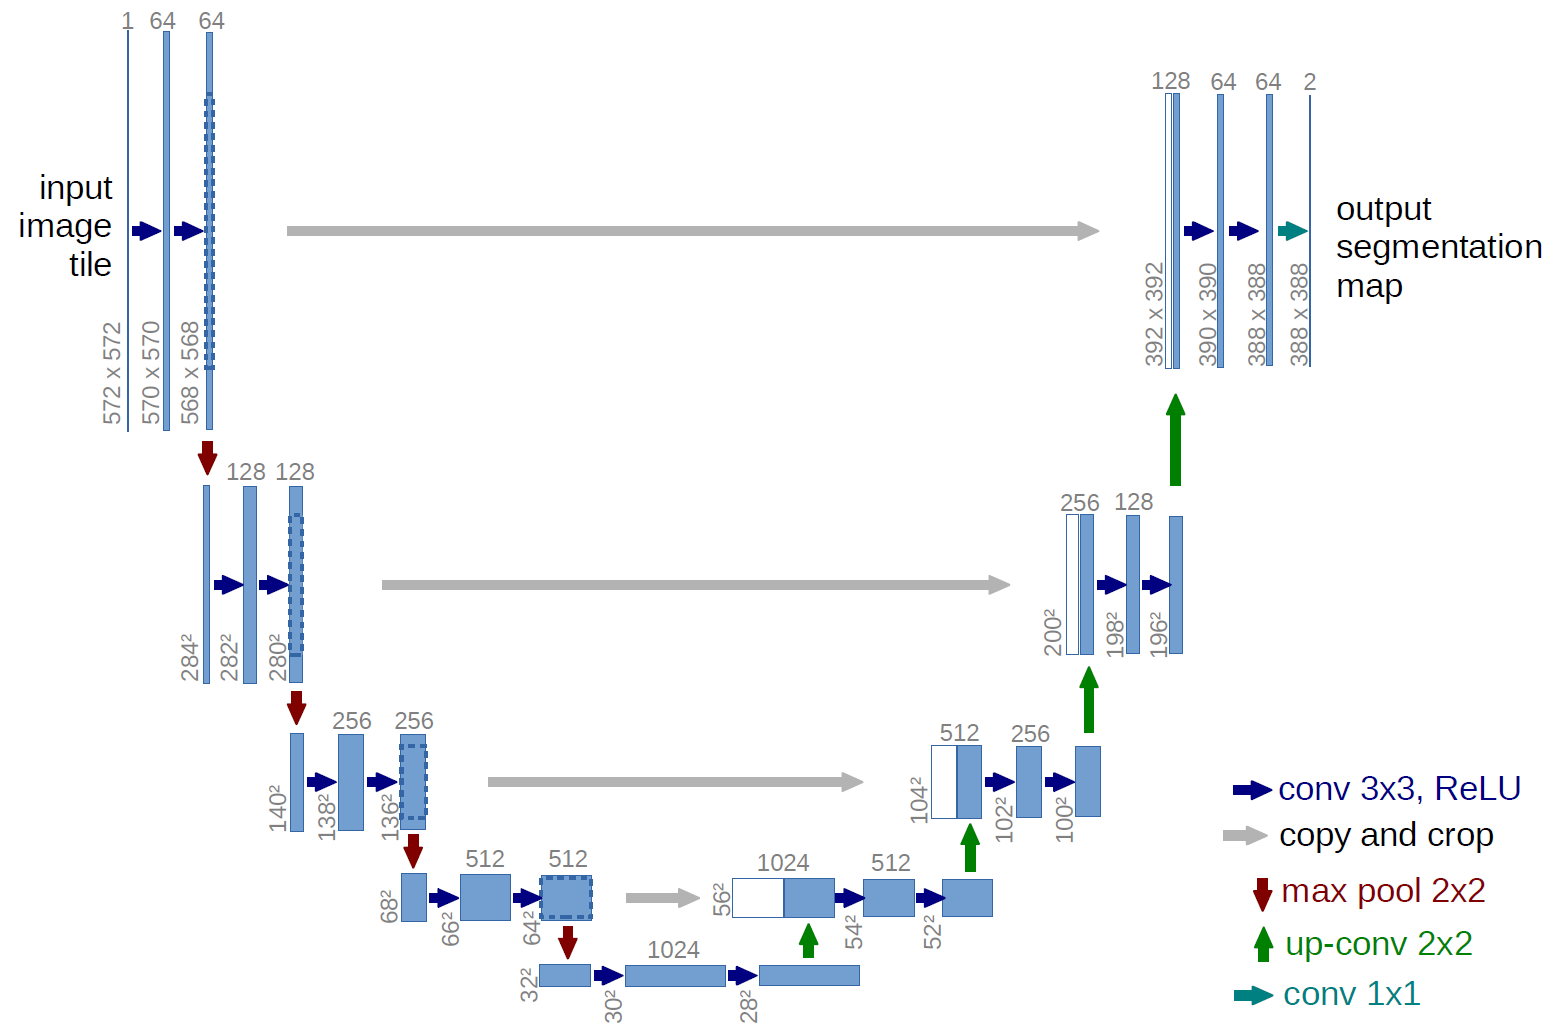
\includegraphics[width=\textwidth]{images/unet.png}
  \caption{Original U-Net architecture \cite{ronneberger2015unet}}
\end{figure}
\\\\
However, Ho et al. \cite{ho2020denoising} made some changes to the original U-Net architecture. \\
First, they state that they used 4 feature map resolutions for their $32 \times 32$ resolution model, and 6 for the $256 \times 256$ resolution model. For each of these feature maps, they used two convolutional residual blocks similar of those of a Wide ResNet \cite{zagoruyko2017wide} consisting of a convolutional layer, a ReLU activation function, a convolutional layer, a group normalisation layer, and another ReLU activation function. \\ 
The "residual" part of the block comes from the fact that the result at the end of the block on the encoder side is concatenated with the result at the end of the block on the decoder side in order to consider features that could have been lost during the downsampling. \cite{lai2022rethinking} \\
They used group normalisation \cite{wu2018group} rather than weight normalisation \cite{salimans2016weight}, which is a normalisation technique that divides the channels into groups and computes the mean and standard deviation for each group \cite{ho2020denoising}. \\
Finally, they state that they used self-attention layers from the Transformer architecture \cite{vaswani2023attention} at the $16 \times 16$ resolution between the two convolutional residual blocks. \cite{ho2020denoising}
\\\\
Since the model needs to be able to predict the noise at any timestep $t$, the authors added a time embedding to the input of the network using the sinusoidal positional embedding from the Transformer architecture \cite{vaswani2023attention}, which allows the parameters to be shared across all timesteps. \\
The sinusoidal positional embedding is given by \cite{vaswani2023attention}:
\begin{align}
  PE_{(pos, 2i)} &= \sin \left( \frac{pos}{10000^{2i/d_{model}}} \right) \\
  PE_{(pos, 2i+1)} &= \cos \left( \frac{pos}{10000^{2i/d_{model}}} \right) \\
  \text{where } \qquad & pos \text{ is the position and } i \text{ is the dimension} \notag
\end{align}
\\\\
Ho et al. \cite{ho2020denoising} present two algorithms: one for training the model and one for sampling from the model:
\\
\begin{minipage}{0.49\textwidth}
  \begin{algorithm}[H]
    \centering
    \caption{Training}\label{alg:training}
    \begin{algorithmic}[1]
      \Repeat
      \State $x_0 \sim q(x_0)$
      \State $t \sim$ Uniform$(\{1,\ldots, T\})$
      \State $\epsilon \sim \mathcal{N}(0, I)$
      \State Take gradient descent step on:
      \State \quad $\nabla_\theta \| \epsilon - \epsilon_\theta \left( \sqrt{\bar{\alpha}_t} x_0 + \sqrt{1 - \bar{\alpha}_t} \epsilon, t \right) \|^2$
      \Until converged
    \end{algorithmic}
  \end{algorithm}
\end{minipage}
\hfill
\begin{minipage}{0.49\textwidth}
  \begin{algorithm}[H]
    \centering
    \caption{Sampling}\label{alg:sampling}
    \begin{algorithmic}[1]
      \State $x_T \sim \mathcal{N}(0, I)$
      \For{$t = T,\ldots, 1$}
        \State $z \sim \mathcal{N}(0, I)$ if $t > 0$, else $z = 0$
        \State $x_{t-1} = \frac{1}{\sqrt{\alpha_t}} \left( x_t - \frac{1 - \alpha_t}{\sqrt{1 - \bar{\alpha_t}}} \epsilon_\theta (x_t, t) \right) + \sigma_t z $
      \EndFor
      \State \textbf{return} $x_0$
    \end{algorithmic}
  \end{algorithm}
\end{minipage}

\subsection{Score-based formulation}
The DDPM paper \cite{ho2020denoising} allows us to predict either the next denoised image, the mean of the next denoised image or the noise itself. \\
However they mention another formulation of the DDPM model that is equivalent: a score-based generative modeling version
\subsubsection{Score matching}
This formulation uses score matching \cite{hyvarinen2005}, either denoising score matching \cite{vincent2010denoising} or sliced score matching \cite{song2019sliced}. \\
Essentially, score matching avoids optimizing the likelihood which can sometimes be difficult to find because of normalisation constants, and instead optimises a score function which is the gradient of the log-likelihood. \\
Suppose we have a probability density function $p_\theta (x)$ that models an i.i.d. dataset $\{x_i\}_{i=1}^N$ of the p.d.f. $p(x)$. 
\\\\
Let $f_\theta (x)$ be a real valued function which is an unnormalized density function and $Z_\theta = \int e^{-f_\theta (x)} dx$ be the normalisation constant such that $\int p_\theta (x) \; dx = 1$. \\
Then $p_\theta(x)$ is defined as:
\begin{align}
  p_\theta (x) &= \frac{e^{-f_\theta (x)}}{Z_\theta}
\end{align}
However for a lot of models, $Z_\theta$ cannot be computed. \cite{luo2022understanding} \\
\\\\
The score function $s_\theta: \mathbb{R}^D \rightarrow \mathbb{R}^D$ is defined as \cite{song2020generative}: 
\begin{align}
  s_\theta (x) &= \nabla_x \log p(x)
\end{align}
If we try to train a model to optimise this score function, we get:
\begin{align}
  s_\theta (x) &= \nabla_x \log p_\theta(x) \\
  &= \nabla_x \log \frac{e^{-f_\theta (x)}}{Z_\theta} \\
  &= \nabla_x \left( -f_\theta (x) - \log Z_\theta \right) \\
  &= - \nabla_x f_\theta (x) - \nabla_x \log Z_\theta \\
  &= - \nabla_x f_\theta (x)
\end{align}
Since $Z_\theta$ is a constant with respect to $x$, $\nabla_x \log Z_\theta = 0$ which means we don't need to compute the intractable normalisation constant $Z_\theta$. \\
This means we could train the score network $s_\theta$ to match the true score function $s(x) = \nabla_x \log p(x)$. \\
The model should then optimise the following Fisher divergence \cite{hyvarinen2005, luo2022understanding}:
\begin{align}
  \frac{1}{2} \mathbb{E}_{x \sim p(x)} \left[ \| s_\theta (x) - s(x) \|_2^2 \right]
\end{align}
However, since we don't know the true score function $s(x)$ which is the score function of the true data distribution $p(x)$, another formulation was shown by Hyvärinen \cite{hyvarinen2005} to be equivalent: 
\begin{align}
  \mathbb{E}_{x \sim p(x)} \left[ \text{ tr}(\nabla_x s_\theta (x)) + \frac{1}{2} \| s_\theta (x) \|_2^2 \right]
\end{align}
This is the score matching objective we want to minimise. \cite{hyvarinen2005}. \\
It can also be computed using the datapoints with the following formula \cite{hyvarinen2005}:
\begin{align}
  \approx \frac{1}{N} \sum_{i=1}^N \text{ tr}(\nabla_x s_\theta (x_i)) + \frac{1}{2} \| s_\theta (x_i) \|_2^2
\end{align}
A problem that arises with this formulation is that the Jacobian matrix $\nabla_x s_\theta (x)$ is not suitable for deep neural networks as it requires backpropagation to compute all its diagonal elements to find the trace \cite{song2020generative, song2019sliced}. To solve this problem, Song et al. \cite{song2020generative} propose either denoising score matching or sliced score matching.
\\\\
\textbf{Denoising score matching} \cite{vincent2010denoising} is a method that slightly noises a datapoint and then score matches the denoised datapoint. This is done by convolving the true data distribution $p$ with a noising kernel $q_\sigma$ but such that $p(x) \approx q_\sigma (x)$. Given a datapoint $x$, we get a noised datapoint $\tilde{x}$ by sampling from $q_\sigma(\tilde{x} | x)$. \\
The score matching now estimates the score of the noised data distribution $q_\sigma(\tilde{x})$, which leads us to the following objective \cite{song2020generative, vincent2010denoising}:
\begin{align}
  \frac{1}{2} \mathbb{E}_{q_\sigma(\tilde{x} | x) p(x)} \left[ \| s_\theta (\tilde{x}) - \nabla_x \log q_\sigma(\tilde{x} | x) \|_2^2 \right]
\end{align}
\\\\
\textbf{Sliced score matching} \cite{song2019sliced} projects the vectors of the vector field $s_\theta (x)$ onto random directions to obtain a scalar field. This will approximate the trace of the Jacobian matrix and it becomes much easier to compute. \cite{song2020generative} \\
We get the following objective \cite{song2019sliced}:
\begin{align}
  \mathbb{E}_{p_v} \mathbb{E}_{x \sim p(x)} \left[ v^T \nabla_x s_\theta (x) \, v + \frac{1}{2} \| s_\theta (x) \|_2^2 \right]
\end{align}
The approximation of the Jacobian matrix $v^T \nabla_x s_\theta (x) \, v$ can be rewritten as \cite{song2019sliced}:
\begin{align}
  v^T \nabla_x s_\theta (x) \, v &= v^T \nabla_x (v^T s_\theta (x))
\end{align}
The gradient of the inner product $\nabla_x (v^T s_\theta (x))$ requires only one backpropagation pass and requires another inner product with $v^T$ to approximate the trace. \cite{song2019sliced} 

\subsubsection{Sampling}
Using the score function mentioned above, we can sample from the model by using Langevin dynamics \cite{song2020generative, WelTeh2011a}, which will give us the definition of score-based generative modeling. \cite{song2020generative}
\\\\
Let $x_0 \sim \pi (x)$ where $\pi (x)$ is an arbitrary distribution (such as a Gaussian distribution), $\epsilon > 0$ a fixed step size and $z_t \sim \mathcal{N}_D (0, I)$. \\
Using Stochastic Gradient Langevin Dynamics (SGLD) \cite{song2020generative, WelTeh2011a}, we can recursively sample using the following formula:
\begin{align}
  x_t &= x_{t-1} + \frac{\epsilon}{2} \nabla_x \log p(x_{t-1}) + \sqrt{\epsilon} z_t
\end{align}
When $T \rightarrow \infty$ and $\epsilon \rightarrow 0$, the distribution of $x_T$ will converge to the true data distribution $p(x)$ therefore the sample will become one from the true data distribution. \cite{song2020generative,WelTeh2011a} \\
$z_t$ is used to add some Gaussian noise at each step because if there was no stochasticity at each step, the sampling would become deterministic and all the samples would essentially be the same.\\
Since we don't know the true data distribution $p(x)$, we can use the score function $s_\theta (x)$ trained to match the true score function $s(x)$ to sample from the model. \\
\begin{align}
  x_t &= x_{t-1} + \frac{\epsilon}{2} s_\theta (x_{t-1}) + \sqrt{\epsilon} z_t
\end{align}
There is however a problem with this method: the score function is well approximated at high density regions where there are a lot of data points but not at low density regions. \cite{song2020generative} \\
Song and Ermon \cite{song2020generative} show this in figure \ref{} by comparing the real score function $\nabla_x \log p(x)$ and the estimated score function $s_\theta (x)$ for a mixture of two Gaussian distributions.
\begin{figure}[h]
  \begin{center}
    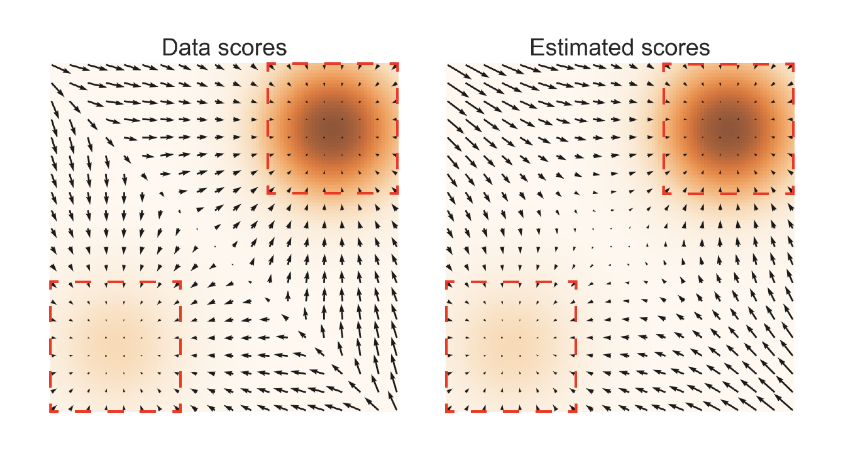
\includegraphics[width= 0.75\textwidth]{images/highlowdensity.png}
    \caption{Data scores represent the real score function $\nabla_x \log p(x)$ and estimated scores reperesent the estimated score function $s_\theta (x)$. We can see that the regions in the red rectangles are the darker high density regions where the score function is well approximated, while the lighter lower density regions outside the red rectangles were not well estimated. \cite{song2020generative}}
  \end{center}
\end{figure}
\\\\
This means that when sampling using Langevin dynamics, the samples will ultimately be incorrect. \cite{song2020generative} 
To correct this, Song and Ermon \cite{song2020generative} use annealed Langevin dynamics. \\
The idea is to add noise to the data points in order to improve the score function estimation in low density regions. \cite{songblog} However adding too much noise will make the score function estimation worse in high density regions. \cite{songblog}. \\
Therefore, they control the amount of noise added using a scale of differents standard deviations $\sigma_i$ with $i = 1, 2, ..., L$ such that $\sigma_1 < \sigma_2 < ... < \sigma_L$. \cite{songblog,song2020generative} \\
To sample, the same Langevin dynamics method is used going from $i = L, L-1, ..., 1$ with $\sigma_i$ decreasing at each step. This is the annealed Langevin dynamics method they used, and the results can be seen in figure \ref{}, where we clearly see that the annealed Langevin dynamics samples are much more similar to the original data samples than the simple Langevin dynamics samples. \cite{songblog,song2020generative} \\ 
\begin{figure}[h]
  \begin{center}
    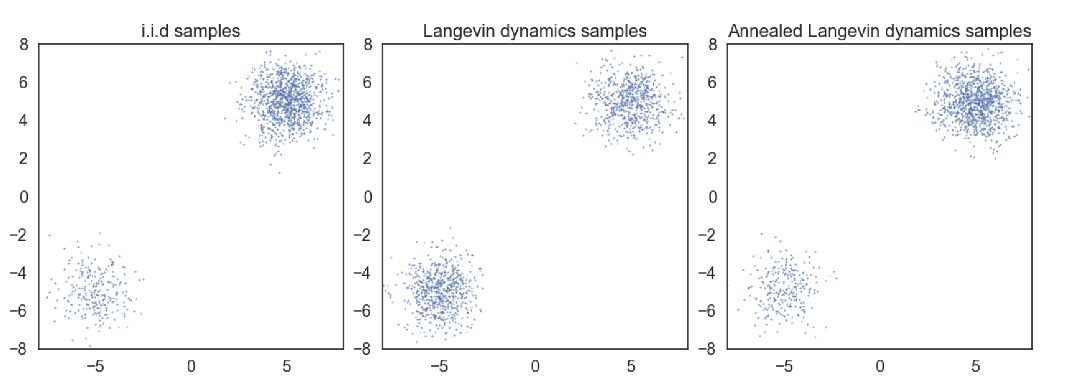
\includegraphics[width=\textwidth]{images/samples.png}
    \caption{Left: Samples from data distribution. Middle: Samples from model using Langevin dynamics. Right: Samples from model using annealed Langevin dynamics. \cite{song2020generative}} 
  \end{center}
\end{figure}
\subsubsection{Noise Conditional Score Networks}
Noise Conditional Score Networks (NCSN) are a score-based generative model that use a neural network to estimate the score function of the previously mentioned noised distribution and then use annealed Langevin dynamics to sample from the model. \cite{song2020generative}
\\\\
Given the increasing sequence of standard deviations $\sigma_i$ with $i = 1, 2, ..., L$, the perturbed data distribution is defined as \cite{song2020generative}:
\begin{align}
  q_{\sigma_i}(x) &= \int p(t) \, \mathcal{N}(x; t, \sigma_i^2) \; dt
\end{align}
Song and Ermon \cite{song2020generative} then define the Noise Conditional Score Network $s_\theta$ that estimates the scores of all the perturbed data distributions $q_{\sigma_i}(x)$ given a data point $x$:
\begin{align}
  s_\theta : \mathbb{R}^D &\times \mathbb{R} \rightarrow \mathbb{R}^D \\
  s_\theta (x, \sigma) &\approx \nabla_x \log q_\sigma (x) \qquad \forall \sigma \in \{ \sigma_1, \sigma_2, ..., \sigma_L \}
\end{align}
To train the NCSN, the authors chose denoising score matching \cite{vincent2010denoising} as its goal is to estimate the score function of a noised data distribution while being quicker than sliced score matching \cite{song2019sliced}. \cite{song2020generative}
\\\\
Let $q_\sigma (\tilde{x} | x) = \mathcal{N}(\tilde{x} | x, \sigma^2, I)$ be the noise distribution that noised the data point $x$ to get the noised data point $\tilde{x}$. \\
Its score function is given by \cite{song2020generative}:
\begin{align}
  \nabla_{\tilde{x}} \log q_\sigma (\tilde{x} | x) &= - \frac{\tilde{x} - x}{\sigma^2} 
\end{align}
Let $\lambda (\sigma_i)$ be a positive coefficient function, often chosen to be $\lambda (\sigma_i) = \sigma_i^2$ \cite{songblog, song2020generative} \\
The denoising score matching objective is given by \cite{song2020generative}:
\begin{align}
  \mathcal{L}(\theta, \{ \sigma_i \}_{i=1}^L) &= \frac{1}{2L} \sum^L_{i=1} \lambda(\sigma_i) \, \mathbb{E}_p(x) \mathbb{E}_{\tilde{x} \sim \mathcal{N}(x, \sigma^2 I)} \left[ \| s_\theta (\tilde{x}, \sigma_i) + \frac{\tilde{x} - x}{\sigma_i^2} \|_2^2 \right]
\end{align}
\\\\
To sample from the model, Song and Ermon \cite{song2020generative} define an algorithm that uses the previously mentioned annealed Langevin dynamics:
\begin{algorithm}[H]
  \centering
  \caption{Sampling from NCSN}\label{alg:ncsn}
  \begin{algorithmic}[1]
    \Require $\{\sigma_i\}_{i=1}^L$, $\epsilon$, $T$ 
    \State $\tilde{x}_0 \sim \pi(x)$
    \For{$i = 1, 2, ..., L $}
      \State $\alpha_i \leftarrow \epsilon \cdot \sigma_i^2 / \sigma_L^2$
      \For{$t = 1, 2, ..., T$}
        \State $z_t \sim \mathcal{N}(0, I)$
        \State $\tilde{x}_t \leftarrow \tilde{x}_{t-1} + \frac{\alpha_i}{2} s_\theta (\tilde{x}_{t-1}, \sigma_i) + \sqrt{\alpha_i} z_t$
      \EndFor
      \State $\tilde{x}_0 \leftarrow \tilde{x}_T$
    \EndFor
    \State \textbf{return} $\tilde{x}_T$
  \end{algorithmic}
\end{algorithm}


\subsubsection{Equivalence between DDPM and NCSN}
Ho et al.'s DDPM paper \cite{ho2020denoising} showed that the DDPM model is equivalent to the NCSN model with denoising score matching and annealed Langevin dynamics. \\
This can be seen by the fact that sampling algorithm \ref{} of the DDPM paper is in fact very similar to the sampling algorithm \ref{} of the NCSN paper, but rather than estimating a score, the DDPM model estimates the noise. \cite{ho2020denoising} \\
Similarly, the score function $s_\theta (x, \sigma)$ can be rewritten in terms of the DDPM's forward process as \cite{weng2021diffusion}:
{
  \allowdisplaybreaks
  \begin{align}
    s_\theta (x, \sigma) \approx \nabla_x \log q_\sigma (x) &\Leftrightarrow s_\theta (x_t, t) \approx \nabla_{x_t} \log q(x_t) \\
    &= \mathbb{E}_{q (x_0)} \left[ \nabla_{x_t} \log q(x_t \, | \, x_0) \right] \\
    &= \mathbb{E}_{q (x_0)} \left[ \nabla_{x_t} \log \mathcal{N} (\sqrt{\bar{\alpha}_t} x_0, (1 - \bar{\alpha}_t) I) \right] \\
    &= \mathbb{E}_{q (x_0)} \left[ \nabla_{x_t} \log e^{- \frac{1}{2} \left( \frac{x_t - \sqrt{\bar{\alpha}_t} x_0}{\sqrt{1 - \bar{\alpha}_t}} \right)^T \left( \frac{x_t - \sqrt{\bar{\alpha}_t} x_0}{\sqrt{1 - \bar{\alpha}_t}} \right)} \right] \\
    &= \mathbb{E}_{q (x_0)} \left[ \Sigma^{-1} (x_t - \sqrt{\bar{\alpha}_t} x_0) \right] \\
    &= \mathbb{E}_{q (x_0)} \left[ \Sigma^{-1} \left(x_t - \sqrt{\bar{\alpha}_t} \left( \frac{x_t - \sqrt{1 - \bar{\alpha}_t} \epsilon_\theta}{\sqrt{\bar{\alpha}_t}} \right) \right) \right] \\
    &= \mathbb{E}_{q (x_0)} \left[ \Sigma^{-1} \left( \sqrt{1 - \bar{\alpha}_t} \epsilon_\theta \right) \right] \\
    &= - \frac{1}{1 - \bar{\alpha}_t}  \sqrt{1 - \bar{\alpha}_t} \epsilon_\theta \\
    &= - \frac{\epsilon_\theta}{\sqrt{1 - \bar{\alpha}_t}}
  \end{align}
  We can see that this quantity is used in sampling algorithm \ref{} of the DDPM paper \cite{ho2020denoising}. 
}



\newpage
\section{Improvements upon DDPMs}

As mentioned previously, the DDPM paper \cite{ho2020denoising} had certain choices that limited its performance.\\
Several papers \cite{nichol2021improved, song2022denoising} following it have improved upon the original DDPM in various ways.

\subsection{Improved likelihood}
Ho et al. \cite{ho2020denoising} admit that their model, despite its high sample quality, did not have a competitive log-likelihood in comparison to other likelihood-based models such as VAEs and autoregressive models \cite{nichol2021improved}
\\\\
The \textit{Improved Denoising Diffusion Probabilistic Models} paper published by Nichol et al. \cite{nichol2021improved} in 2021 implemented certain changes in order to improve the log-likelihood of the model not only on simpler datasets such as CIFAR-10 \cite{cifar10} that the original DDPM was trained on, but also on more complex datasets such as ImageNet. \cite{kingma2022autoencoding, oord2016conditional, nichol2021improved}.
\\\\
In order to improve the log-likelihood, Nichol et al. \cite{nichol2021improved} started by investigating the fixed variance $\Sigma_\theta (x_t, t) = \sigma_t^2 I = \beta_t I$ of the original DDPM and whether or not it could be worth learning it. \\
Recall that Ho et al. \cite{ho2020denoising} saw no difference in sample quality when using a learned variance $\tilde{\beta}_t$ and therefore opted for using the fixed variance $\beta_t$. \\
Nichol et al. \cite{nichol2021improved} came to the same conclusion, finding that as the number of steps $T$ increased (the authors also mentioned that they used $T = 4000$ for their models rather than $T = 1000$ from the original paper), the difference between $\beta_t$ and $\tilde{\beta}_t$ remained very small. However, they were still interested in the possibility of learning the variance in order to improve the log-likelihood. \cite{nichol2021improved}. \\
For this, they used an interpolation approach, where they parametrised the variance as an interpolation between the fixed variance $\beta_t$ and a learned variance $\tilde{\beta}_t$ in the $\log$ domain, with $v$ an output vector from the model containing one component per dimension:
\begin{align}
  \Sigma_\theta (x_t, t) &= \exp \left( v \log \beta_t + (1 - v) \log \tilde{\beta}_t \right)
\end{align}
As the simplified training objective $L_{\text{simple}}$ used in the original DDPM paper \cite{ho2020denoising} did not include the variance, Nichol et al. \cite{nichol2021improved} introduced a new training objective $L_{\text{hybrid}}$, defined as:
\begin{align}
  L_{\text{hybrid}} &= L_{\text{simple}} + \lambda L_{\text{VLB}}
\end{align}
with $\lambda = 0.001$ in order to keep $L_{\text{simple}}$ as the main training objective. \cite{nichol2021improved}
\\\\
At first, they found that the hybrid objective $L_{\text{hybrid}}$ achieved a better log-likelihoods and was easier to optimise than just $L_{\text{VLB}}$, contrary to what they had expected. \cite{nichol2021improved} \\
However, they obtained the best log-likelihoods by optimising $L_{\text{VLB}}$ directly but with importance samping, which is a technique where samples of a difficult distribution are taken from a distribution that is easier to compute and then the original distribution is approximated by weighted samples. \cite{nichol2021improved}
\\\\
They defined it as:
\begin{align}
  L_{\text{VLB}} &= \mathbb{E}_{t \sim p_t} \left[ \frac{L_t}{p_t} \right]
  &\text{where } p_t \propto \sqrt{\mathbb{E}\left[ L_t^2 \right]} \text{ and } \sum p_t = 1
\end{align}
\\
Another change that Nichol et al. \cite{nichol2021improved} made was to use a cosine noising schedule rather than the linear noising schedule used in the original DDPM paper \cite{ho2020denoising}. \\
They explain this change by the fact that towards the end of the forward process, the image is already very noisy and yet more noise is added while not really improving the model, particularly for $32 \times 32$ and $64 \times 64$ images. \cite{nichol2021improved} \\
In effect, the input images get destroyed by noise very quickly with the linear noising schedule converging to zero rapidly. \cite{nichol2021improved}
\\\\
They define the cosine schedule as:
\begin{align}
  f(t) &= \cos \left( \frac{\frac{t}{T} + s}{1 + s} \cdot \frac{\pi}{2} \right)^2 \\
  \bar{\alpha}_t &= \frac{f(t)}{f(0)} \\
  \beta_t &= 1 - \frac{\bar{\alpha}_t}{\bar{\alpha}_{t-1}}
\end{align}
$T$ is the total number of timesteps, $t$ is the timestep and $s$ is a small offset used to prevent $\beta_t$ from being too small when $t = 0$ in order to allow the noise $\epsilon$ to be predicted more accurately at the beginning of the process. \cite{nichol2021improved}.
\\\\
With these changes, Nichol et al. \cite{nichol2021improved} were able to achieve a negative log-likelihood (NLL) of $2.94$ bits/dim on CIFAR-10 \cite{cifar10} and $3.53$ bits/dim on ImageNet \cite{oord2016conditional}, compared to the original DDPM paper \cite{ho2020denoising} which had a NLL of $3.70$ on CIFAR-10 and $3.77$ on ImageNet. \cite{nichol2021improved}.
\\\\
\begin{figure}[h]
  \begin{center}
    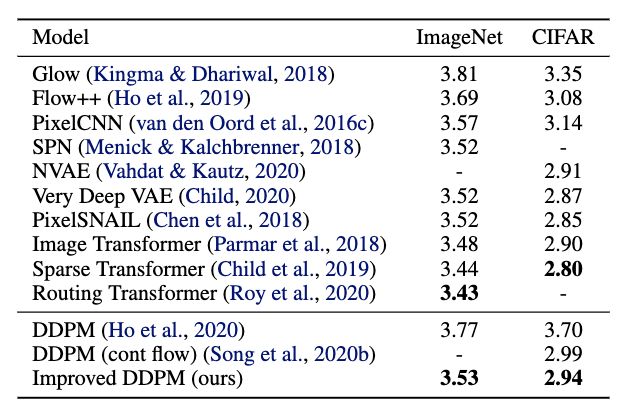
\includegraphics[width= 0.6\textwidth]{images/comparison.png}
    \caption{Comparison of NLLs of different models \cite{nichol2021improved}}
  \end{center}
\end{figure}
\\\\
Moreover, Nichol et al. \cite{nichol2021improved} were able to improve sampling speed due to the aforementioned changes, even though they trained their model with $T = 4000$ timesteps. \\
They were able to train their model with $4000$ timesteps, but use only $100$ timesteps for sampling which brought them near-optimal FID (Fréchet Inception Distance) scores when using the $L_{\text{hybrid}}$ training objective. \cite{nichol2021improved} \\
They had tried to reduce the number of sampling steps with the original fixed variance versions from the DDPM paper \cite{ho2020denoising} but found that the sample quality degraded a lot more. \cite{nichol2021improved}

\newpage

\subsection{Denoising Diffusion Implicit Models (DDIMs)}
As mentioned previously, the DDPM paper \cite{ho2020denoising} has a forward process and a reverse process which are both Markov processes. \\
While the forward process can be easily calculated for a specific timestep $t$ with equation \ref{eq:}, the reverse process still requires 1000 timesteps in the case of Ho et al.'s \cite{ho2020denoising} model, and Nichol et al.'s model requires 100 and 4000 timesteps for sampling and training respectively. \cite{nichol2021improved} \\
This is time-consuming and computationally expensive compared to GANs which only require one forward pass through the network rather than thousands to produce a sample. \cite{song2022denoising}
\\\\
To address this issue, Song et al. \cite{song2022denoising} introduced the Denoising Diffusion Implicit Models (DDIMs) in 2020. \\
The main objective of DDIMs was to accelerate sampling by making the forward process non-Markovian, which would allow the reverse process to require less iterations. \cite{song2022denoising}
\\\\
Song et al. \cite{song2022denoising} define a family $\mathcal{Q}$ of forward processes, each indexed by $\sigma \in \mathbb{R}^T_+$:
\begin{align}
  q_{\sigma}(x_{1:T}| \, x_0) &= q_{\sigma}(x_T | \, x_0) \prod_{t=2}^{T} q_{\sigma}(x_{t-1}| \, x_t, x_0)
\end{align}
where
\begin{align}
  q_{\sigma}(x_T | \, x_0) &= \mathcal{N}(\sqrt{\alpha_T} x_0, (1 - \alpha_T) I)
\end{align}
and for all $t > 1$:
\begin{align}
  q_{\sigma}(x_{t-1} | \, x_t, x_0) &= \mathcal{N}\left( \sqrt{\alpha_{t-1}} x_0 + \sqrt{1 - \alpha_{t-1} - \sigma_t^2} \cdot \frac{x_t - \sqrt{\alpha_t} x_0}{\sqrt{1 - \alpha_t}}, \: \sigma_t^2 I \right)
\end{align}
It is interesting to note that when $\sigma_t^2 = (1 - \alpha_t)(1 - \bar{\alpha}_{t-1})/(1 - \bar{\alpha}_t)$, we obtain equation \ref{eq:}, which was the definition of the forward process in the original DDPM paper \cite{ho2020denoising, song2022denoising}. \\
Song et al. \cite{song2022denoising} also note when $\sigma_t^2 = 0$, then $x_{t-1}$ is fixed and known in advance. \\
Therefore, we can see that as Song et al. \cite{song2022denoising} state, the value of $\sigma$ controls the stochasticity (or more simply, the randomness) of the forward process.
\\\\
The authors use Bayes' rule similarly to the original DDPM paper \cite{ho2020denoising} in equation \ref{eq:}, but instead to find the forward process $q_\sigma(x_t | \, x_{t-1}, x_0)$:
\begin{align}
  q_{\sigma}(x_t | \, x_{t-1}, x_0) &= \frac{q_\sigma (x_{t-1} | \, x_t, x_0) \: q_\sigma (x_t | \, x_0)}{q_\sigma (x_{t-1} | \, x_0)}
\end{align}
Since $q_\sigma (x_t | \, x_{t-1}, x_0)$ means that $x_t$ not only depends on $x_{t-1}$ but also on $x_0$, we see that the forward process is no longer Markovian, which was what the authors were aiming to achieve. \cite{song2022denoising}
\\\\
However, since the reverse process in the original DDPM paper \cite{ho2020denoising} was anestimation of the forward process which was Markovian, a new reverse process was defined. \\
Their idea of the reverse process is to sample an image $x_T$ like in the original DDPM paper \cite{ho2020denoising}, predict $x_0$ from $x_T$ and then use this prediction of $x_0$ to sample $x_{T-1}$. \cite{song2022denoising} \\
This is repeated until we reach $x_1$ and then $x_0$ is predicted from $x_1$. \cite{song2022denoising} \\
Similar to equation \ref{eq:} from the DDPM paper, Song et al. \cite{song2022denoising} define the prediction of $x_0$ from $x_t$ as:
\begin{align}
  f_\theta^{(t)} (x_t) &= \frac{x_t - \sqrt{1 - \bar{\alpha}_t} \: \epsilon(x_t, t)}{\sqrt{\bar{\alpha}_t}}
\end{align}
Given this, the reverse process is defined as \cite{song2022denoising}:
\begin{align}
  p_\theta (x_T) &= \mathcal{N}_D(0, I) \\
  p_\theta^{(t)} (x_{t-1} | \, x_t) &= \begin{cases}
    \mathcal{N}(f_\theta^{(1)}(x_{1}), \sigma_1^2 I) & \text{if } t = 1 \\
    q_\sigma(x_{t-1} | \, x_t, f_\theta^{(t)}(x_t)) & \text{if } t > 1
  \end{cases}
\end{align}
Therefore, $x_{t-1}$ is sampled from $x_t$ \cite{song2022denoising}: 
\begin{align}
  x_{t-1} &= \sqrt{\alpha_{t-1}} \left( \frac{x_t - \sqrt{1 - \bar{\alpha}_t} \: \epsilon(x_t, t)}{\sqrt{\bar{\alpha}_t}} \right) + \sqrt{1 - \alpha_{t-1} - \sigma_t^2} \cdot \epsilon_\theta (x_t, t) + \sigma_t \epsilon_t
\end{align}
In order to train the model, Song et al. \cite{song2022denoising} define the following \textit{variational inference objective}:
\begin{align}
  J_\sigma & (\epsilon_\theta) = \mathbb{E}_{q_\sigma (x_{0:T})} \left[ \log q_\sigma (x_{1:T} | \, x_0) - \log p_\theta (x_{0:T}) \right] \\
  &= \mathbb{E}_{q_\sigma (x_{0:T})} \left[ \log q_\sigma (x_T | \, x_0) + \sum_{t=2}^{T} \log q_\sigma (x_{t-1} | \, x_t, x_0) - \sum_{t=1}^{T} \log p_\theta^{(t)} (x_{t-1} | \, x_t) - \log p_\theta (x_T) \right]
\end{align}
This would mean that for different choices of $\sigma$, we would have a different objective to optimise. \cite{song2022denoising} \\
However, the authors \cite{song2022denoising} prove that $J_\sigma$ is in fact equivalent to $L_\gamma$ for certain choices of $\gamma$, where $L_\gamma$ is defined as:
\begin{align}
  L_\gamma (\epsilon_\theta) &= \sum_{t=1}^{T} \gamma_t \mathbb{E}_{x_0 \sim q(x_0), \epsilon_t \sim \mathcal{N}(0, I)}  \left[ \| \epsilon_\theta^{(t)} (\sqrt{\alpha_t} x_0 + \sqrt{1 - \alpha_t} \epsilon_t) - \epsilon_t \|_2^2 \right]
\end{align}
where $\gamma$ is a vector of length $T$ with positive values that depend on $\alpha$. \\
We easily see that when $\gamma = 1$, we get $L_1$ which is the training objective from the original DDPM paper. \cite{ho2020denoising, song2022denoising} \\
Song et al. prove that
\begin{align}
  \forall \sigma > 0, \, \exists \, \gamma \in \mathbb{R}_+^T \text{ and } \exists \, C \in \mathbb{R} \text{ s.t. } J_\sigma = L_\gamma + C
\end{align}
This means that the optimal solution for $J_\sigma$ is the same as the optimal solution for $L_1$, which means that the training objective for DDIMs can be kept the same as the one for DDPMs if the parameters being trained $\theta$ are not the same for all timesteps. \cite{song2022denoising}
\\\\
In order to speed up the sampling process, Song et al. \cite{song2022denoising} skip some timesteps in the reverse process. \\
To do this, the forward process is redefined on a subset of timesteps of size $S$, $\left\{ x_{\tau_1}, ..., x_{\tau_S} \right\}$ and such that $q(x_{\tau_i} | \, x_0) = \mathcal{N}(\sqrt{\alpha_{\tau_i}} x_0, (1 - \alpha_{\tau_i})I)$ \\
Since this is a subset of the timesteps, the training can be done all timesteps and the sampling can be done on the subset. \cite{song2022denoising}
\\\\
With the same amount of training timesteps $T = 1000$ and the same training objective as the DDPM paper \cite{ho2020denoising}, Song et al. \cite{song2022denoising} were able to achieve solid FID scores on CIFAR-10 \cite{cifar10} and CelebA \cite{liu2015faceattributes} datasets, with far fewer sampling timesteps, ranging from $10$ to $100$ timesteps. \cite{song2022denoising} \\
A new hyperparameter $\eta \in \mathbb{R}_+$ is introduced to control the interpolation between the DDPM $\sigma$ and the deterministic $\sigma$ of the DDIM. \cite{song2022denoising}:
\begin{align}
  \sigma_{\tau_i} (\eta) &= \eta \sqrt{\frac{1 - \alpha_{\tau_{i-1}}}{1 - \alpha_{\tau_i}}} \sqrt{1 - \frac{\alpha_{\tau_i}}{\alpha_{\tau_{i-1}}}}
\end{align}
The results obtained by Song et al. \cite{song2022denoising} show that the DDIM outperformed the DDPM for 10, 20, 50, 100 and 1000 timesteps and was only slightly worse at $1000$ timesteps and $\sigma_{\tau_i} = \hat{\sigma}_{\tau_i} = \sqrt{1 - \alpha_{\tau_i} / \alpha_{\tau_{i-1}}}$
\\\\
\begin{figure}[h]
  \begin{center}
    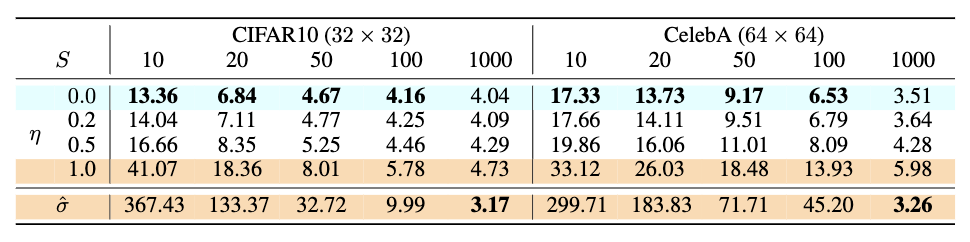
\includegraphics[width=\textwidth]{images/ddim_table.png}
    \caption{Comparison of FID scores (lower is better) of DDPMs and DDIMs trained on $S$ timesteps, $S < T$ and $\eta = 0$ is DDIM, $\eta = 1$ and $\hat{\sigma}$ are DDPMs \cite{song2022denoising}}
  \end{center}
\end{figure}
\\\\


\subsection{Guidance}
Recall that when sampling from a DDPM or a DDIM, we start with an image of Gaussian noise $x_T$ and we denoise the image until we get some image $x_0$ that resembles an image from the original dataset. We may however be interested in sampling something specific; for instance, from some text. \\
In this case it is helpful to guide the denoising process towards whatever we specified.
\subsubsection{Classifier guidance}
Classifier guidance was introduced by Dhariwal and Nichol in their \textit{Diffusion Models Beat GANs on Image Synthesis} paper \cite{dhariwal2021diffusion} in order to improve the samples generated. \\
To do this, they trained a classifier $p_\Phi (y \, | \, x_t, t)$ on noisy images \cite{dhariwal2021diffusion} since pre-trained classifiers were are generally trained on dataset images and not on noised ones. \\
The reverse process is then guided towards a class $y$ using the gradient $\nabla_{x_t} \log p_\Phi (y \, | \, x_t, t)$. \cite{dhariwal2021diffusion}
The authors prove \cite{dhariwal2021diffusion} that if we have a reverse process such as that from the DDPM $p_\theta (x_t, x_{t+1})$, to condition it on class $y$, we can sample from the following process instead:
\begin{align}
  p_{\theta, \Phi} (x_t \, | \, x_{t+1}, y) &= Z p_\theta (x_t \, | \, x_{t+1}) \, p_\Phi(y \, | \, x_t)
\end{align}
where $Z$ is a normalization constant.



\subsubsection{Classifier-free guidance}
Despite the impressive performance of the \textit{ablated diffusion model} that used classifier guidance, Ho and Salimans made an improvement by using classifier-free guidance. \cite{ho2022classifierfree}

\newpage
\section{Comparison with other diffusion models}

\newpage
\section{Implementation}

\newpage
\section{Conclusion}

\newpage
\appendix
\section{Convolution of two Gaussian distributions}
Equation \ref{eq:} had given us:
\begin{align*}
  x_t &= \sqrt{\alpha_t \alpha_{t-1}} x_{t-2} + \mathcal{N}\left(0, \alpha_t\left(1 - \alpha_{t-1}\right)I \right) + \mathcal{N}\left(0, (1 - \alpha_t) I \right)
\end{align*}
We can find the distribution of the sum of two independant 1D random variables $X \sim \mathcal{N}\left(\mu_X, \sigma_X^2\right)$ and $Y \sim \mathcal{N}\left(\mu_Y, \sigma_Y^2\right)$ as the convolution of two Gaussian distributions.
\\\\
Let $Z = X + Y$ with $X$ and $Y$ independent.
{
  \allowdisplaybreaks
\begin{align*}
  f_Z(z) &= \int_{-\infty}^{\infty} f_X(x) f_Y(z - x) \: dx \\
  &= \int_{-\infty}^{\infty} \frac{1}{\sqrt{2 \pi \sigma_X^2}} \exp \left[{-\frac{(x - \mu_X)^2}{2 \sigma_X^2}} \right] \frac{1}{\sqrt{2 \pi \sigma_Y^2}} \exp \left[{-\frac{(z - x - \mu_Y)^2}{2 \sigma_Y^2}} \right] \: dx \\[10pt]
  &= \frac{1}{2 \pi \sigma_X \sigma_Y} \int_{-\infty}^{\infty} \exp \left[{-\frac{(x - \mu_X)^2}{2 \sigma_X^2}} \right] \exp \left[{-\frac{(z - x - \mu_Y)^2}{2 \sigma_Y^2}} \right] \: dx \\[10pt]
  &= \frac{1}{2 \pi \sigma_X \sigma_Y} \int_{-\infty}^{\infty} \exp\left[{-\frac{(x - \mu_X)^2}{2 \sigma_X^2} - \frac{(z - x - \mu_Y)^2}{2 \sigma_Y^2}} \right] \: dx \\[10pt]
  &= \frac{1}{2 \pi \sigma_X \sigma_Y} \int_{-\infty}^{\infty} \exp\left[{-\frac{x^2 - 2 \mu_X x + \mu_X^2}{2 \sigma_X^2} - \frac{z^2 + x^2 - 2 x z - 2 z \mu_Y + 2 \mu_Y x + \mu_Y^2}{2 \sigma_Y^2}} \right] \: dx \\[10pt]
  &= \frac{1}{2 \pi \sigma_X \sigma_Y} \int_{-\infty}^{\infty} \exp\left[{-\frac{\sigma_Y^2(x^2 - 2 \mu_X x + \mu_X^2)}{2 \sigma_X^2 \sigma_Y^2} - \frac{\sigma_X^2(z^2 + x^2 - 2 x z - 2 z \mu_Y + 2 \mu_Y x + \mu_Y^2)}{2 \sigma_X^2 \sigma_Y^2 }} \right] \: dx \\[10pt]
  &= \frac{1}{2 \pi \sigma_X \sigma_Y} \int_{-\infty}^{\infty} \exp\left[{-\frac{\sigma_Y^2 x^2 - 2 \mu_X \sigma_Y^2 x + \mu_X^2 \sigma_Y^2 + \sigma_X^2 z^2 + \sigma_X^2 x^2 - 2xz\sigma_X^2 + 2 z \mu_Y \sigma_X^2 - 2\mu_Y x \sigma_X^2 + \sigma_X^2 \mu_Y^2}{2 \sigma_X^2 \sigma_Y^2}} \right] \: dx \\[10pt]
  &= \frac{1}{2 \pi \sigma_X \sigma_Y} \int_{-\infty}^{\infty} \exp\left[{-\frac{\left(\sigma_X^2 + \sigma_Y^2\right) x^2 - 2 x \left( \mu_X \sigma_Y^2 + z \sigma_X^2 - \mu_Y \sigma_X^2 \right) + \sigma_X^2 \left( z - \mu_Y \right)^2 + \mu_X^2 \sigma_Y^2}{2 \sigma_X^2 \sigma_Y^2}} \right] \: dx \\[10pt]
  &\text{Let $\sigma_Z = \sqrt{\sigma_X^2 + \sigma_Y^2}$}. \\
  &= \frac{1}{\sqrt{2 \pi} \frac{\sigma_X \sigma_Y}{\sigma_Z}} \frac{1}{\sqrt{2 \pi} \sigma_Z} \int_{-\infty}^{\infty} \exp\left[{-\frac{x^2 - 2x \frac{\sigma_X^2 (z - \mu_Y) + \sigma_Y^2 \mu_X}{\sigma_Z^2} + \frac{\sigma_X^2 \left( z - \mu_Y \right)^2 + \mu_X^2 \sigma_Y^2}{\sigma_Z^2}}{2 \left(\frac{\sigma_X \sigma_Y}{\sigma_Z}\right)^2}} \right] \: dx \\[10pt]
  &= \frac{1}{\sqrt{2 \pi} \frac{\sigma_X \sigma_Y}{\sigma_Z}} \frac{1}{\sqrt{2 \pi} \sigma_Z} \int_{-\infty}^{\infty} \exp\left[{-\frac{\left( x - \frac{\sigma_X^2 (z - \mu_Y) + \sigma_Y^2 \mu_X}{\sigma_Z^2}\right)^2 - \left( \frac{\sigma_X^2 (z - \mu_Y) + \sigma_Y^2 \mu_X}{\sigma_Z^2} \right)^2 + \frac{\sigma_X^2 (z - \mu_Y)^2 + \sigma_Y^2 \mu_X^2}{\sigma_Z^2}}{2 \left(\frac{\sigma_X \sigma_Y}{\sigma_Z}\right)^2}} \right] \: dx  \\[10pt]
  &= \int_{-\infty}^{\infty} \frac{1}{\sqrt{2 \pi} \frac{\sigma_X \sigma_Y}{\sigma_Z}} \exp\left[{-\frac{\left( x - \frac{\sigma_X^2 (z - \mu_Y) + \sigma_Y^2 \mu_X}{\sigma_Z^2}\right)^2}{2 \left(\frac{\sigma_X \sigma_Y}{\sigma_Z}\right)^2}} \right] \\[10pt]
  & \hspace{3cm} \frac{1}{\sqrt{2 \pi} \sigma_Z} \exp \left[ - \frac{\sigma_Z^2 \left( \sigma_X^2 (z - \mu_Y)^2 + \sigma_Y^2 \mu_X^2 \right) - \left( \sigma_X^2 (z - \mu_Y) + \sigma_Y^2 \mu_X \right)^2}{2 \sigma_Z^2 (\sigma_X \sigma_Y)^2} \right] \: dx  \\[10pt]
  &= \int_{-\infty}^{\infty} \frac{1}{\sqrt{2 \pi} \frac{\sigma_X \sigma_Y}{\sigma_Z}} \exp\left[{-\frac{\left( x - \frac{\sigma_X^2 (z - \mu_Y) + \sigma_Y^2 \mu_X}{\sigma_Z^2}\right)^2}{2 \left(\frac{\sigma_X \sigma_Y}{\sigma_Z}\right)^2}} \right] \frac{1}{\sqrt{2 \pi} \sigma_Z} \exp \left[ - \frac{(z - (\mu_X + \mu_Y))^2}{2 \sigma_Z^2} \right] \: dx  \\[10pt]
  &= \frac{1}{\sqrt{2 \pi} \sigma_Z} \exp \left[ - \frac{(z - (\mu_X + \mu_Y))^2}{2 \sigma_Z^2} \right] \int_{-\infty}^{\infty} \frac{1}{\sqrt{2 \pi} \frac{\sigma_X \sigma_Y}{\sigma_Z}} \exp\left[{-\frac{\left( x - \frac{\sigma_X^2 (z - \mu_Y) + \sigma_Y^2 \mu_X}{\sigma_Z^2}\right)^2}{2 \left(\frac{\sigma_X \sigma_Y}{\sigma_Z}\right)^2}} \right] \: dx  \\[10pt]
  &= \frac{1}{\sqrt{2 \pi} \sigma_Z} \exp \left[ - \frac{(z - (\mu_X + \mu_Y))^2}{2 \sigma_Z^2} \right] \\[10pt]
  &= \mathcal{N}\left(z; \mu_X + \mu_Y, \sigma_X^2 + \sigma_Y^2 \right)
\end{align*}
}
\\
Given this, we can refer back to our case and therefore we find:
\begin{align*}
  x_t &= \sqrt{\alpha_t \alpha_{t-1}} x_{t-2} + \mathcal{N}\left(0, \alpha_t\left(1 - \alpha_{t-1}\right)I \right) + \mathcal{N}\left(0, (1 - \alpha_t) I \right) \\
  &= \sqrt{\alpha_t \alpha_{t-1}} x_{t-2} + \mathcal{N}\left(0, \alpha_t \left((1 - \alpha_{t-1}) + 1 - \alpha_t \right)I \right) 
\end{align*}
%% ----------------------------------------------------------------- %%

\newpage
\printbibliography

\end{document}
